\setcounter{chapter}{2}

\chapter{微分中值定理与导数的应用}

微分学最初是独立于积分学的,因为其自身已经可以解决许多的应用问题。
本章讨论的极值、最值、单调性和曲率等,都是微分学的独立应用,其中
中值定理和Taylor公式又可以说是整个微分学的“制高点”,集成和融汇
了导数与微分的绝大部分思想与概念,正确地理解和熟练掌握这部分的知识
是对微积分有一个全面深刻认识的基础。

\section{微分中值定理}

中值定理在微分学中是一个非常富于技巧性和魅力的领域,我接下来我们所介绍的
从Rolle定理、Lagrange中值定理、Cauchy中值定理到Taylor公式的演进
路径,真正地将微分学推向了发展和应用的顶峰。

\subsection{Rolle定理}

\begin{thx}
	{\bf Fermat引理}:若函数$f(x)$在$x_0$处可导,且在$x_0$的某邻域内,有
	$$f(x)\geq f(x_0)\quad (\mbox{或}\quad f(x)\leq f(x_0))$$
	则$f'(x_0)=0$。
\end{thx}

[证]:设当$x\in U_0(x_0,\delta)$时,总有$f(x)\geq f(x_0)$,则
当$x>x_0$时,总有
$$\df{f(x)-f(x_0)}{x-x_0}\geq 0,$$
而当$x<x_0$时,总有
$$\df{f(x)-f(x_0)}{x-x_0}\leq 0,$$
由极限的保号性,分别令$x\to x_0^+$和$x\to x_0^-$,则有
$$f'(x_0)\geq 0,\quad\mbox{且}\quad f'(x_0)\leq 0,$$
由此即知$f'(x_0)=0$。\hfill$\Box$

\begin{shaded}
	{\bf 关于Fermat和Fermat's Last Theorem}
	
	Pierre de Fermat(1601-1665),法国律师和业余数学家。
	他在数学上的成就不比职业数学家差,他似乎对数论最有兴趣,亦对现代微积分的建立有所贡献。
	\begin{itemize}
% 	  \setlength{\itemindent}{1cm}
	  \item 微积分:Fermat引理给出了求极值的必要条件;
	  \item 将Apollonius of Perga(公元前262-190)的几何分析中用代数
	  方法来重新建立,开辟了{\it 解析几何}之路。
	  (Fermat只使用一轴,只接受正数的答案。后世多以Descartes为解析几何的创立者,
	  主因是Fermat没有发表其作品。)
	  \item 1654年,和Pascal在书信中的讨论,被认为是{\it 概率论}的开端,
	  1656年和概率论的正式创立者Christiaan Huygens(1629-1695)的交流,
	  使后者增加了对概率论的兴趣
	\end{itemize}
	
	\begin{tcolorbox}
		Fermat{\it 小定理}:假设$a\in\mathbb{Z}$,$p$为素数,则$a^p-a$可以整除$p$,
		或者写为
		$$a^p\equiv a(\mathrm{mod}p),$$
		特别低,若$a$不是$p$的倍数,则上式可写为$a^{p-1}\equiv 1(\mathrm{mod} p)$
	\end{tcolorbox}
	
	Fermat小定理是RSA公钥加密体制的理论基础,如果没有公钥加密体制,信息技术将
	不可能呈现今天的面貌。下面的是Fermat最重要的一个猜想,也是最后被证明的一个猜想。
	
	\begin{tcolorbox}
		Fermat{\it 大定理}(也称Fermat最后定理):对于大于$2$的正整数$n$,以下方程
		无正整数解
		$$x^n+y^n=z^n.$$
	\end{tcolorbox}
	
	这个定理造成了数学史上最大的悬案:1637年,费马在阅读丢番图《算术》拉丁文译本时,
	曾在第11卷第8命题旁写道:
	{\it 将一个立方数分成两个立方数之和,或一个四次幂分成两个四次幂之和,
	或者一般地将一个高于二次的幂分成两个同次幂之和,这是不可能的。
	关于此,我确信已发现了一种美妙的证法,可惜这里空白的地方太小,写不下。}
	
	一直被称为“Fermat猜想”,直到英国数学家Andrew John Wiles及其学生Richard
	Taylor于1995年将他们的证明出版后,才称为“Fermat大定理”。
	经过数学家们三个多世纪的努力,猜想才变成了定理。在冲击这个数论世纪难题的过程中,
	无论是不完全的还是最后完整的证明,都给数学界带来很大的影响;很多的数学结果、
	甚至数学分支在这个过程中诞生了,包括代数几何中的{\it 椭圆曲线}和{\it 模形式},
	以及{\it	Galois理论}和{\it Hecke代数}等。这也令人怀疑
	当初费马是否真的找到了正确证明。
	
	\begin{itemize}
	  \setlength{\itemindent}{1cm}
	  \item 1770年,Euler证明 $n=3$时定理成立
	  \item 1823年,Legendre证明$n=5$时定理成立
      \item 1832年,Dirichlet试图证明$n=7$失败,但证明$n=14$时定理成立
	  \item 1839年,Gabriel Lamé证明$n=7$时定理成立
	  \item 1850年,Ernst Eduard Kummer证明$2<n<100$时除$37$、$59$、$67$三数外定理成立
	  \item 1955年,Harry Vandiver以电脑计算证明了对所有不超过$2521$的素数定理成立
	  \item 1976年,Samuel Wagstaff以电脑计算证明对所有不超过$125000$的素数定理成立
	  \item 1985年,电脑计算证明了对所有小于$4$百万的素数定理成立
	  \item 1987年,格朗维尔以电脑计算证明了$2<n<10^{{1800000}}$时定理成立
	  \item 1995年,Wiles证明$n>2$时定理成立。
	\end{itemize}
	
	Wiles证明Fermat大定理的过程亦甚具戏剧性。他用了七年时间,在不为人知的情况下,
	得出了证明的大部分;然后于1993年6月在一个学术会议上宣布了他的证明,并瞬即
	成为世界头条。但在审批证明的过程中,专家发现了一个极严重的错误。Wiles和他的学生Taylor
	然后用了近一年时间尝试补救,终在1994年9月以一个之前Wiles抛弃过的方法得到成功。
	
	为什么Fermat大定理在数学史上的地位如此重要?有三个主要的原因:一是问题基本,长时间
	(350年)悬而未决,吸引了众多数学大师对其加以研究;二是研究问题的过程中产生了新的思想和方法,
	带动了数学很多领域的发展;三是涉及Taniyama-Shimura theorem({\it 谷山—志村猜想}),
	是现代数学大热门Langlands program({\it 朗兰兹纲领})的重要组成部分。1967年提出的
	Langlands program指出三个相对独立发展起来的数学分支:数论、代数几何和群表示论,
	实际上是密切相关的,而连接这些数学分支的纽带是一些特别的函数,被称为L-函数。
	L-函数可以说是Langlands program的中心研究对象。数学界著名的七个
	{\it “千禧年大奖问题”}(Millennium Prize Problems)中有两个就是关于L-函数的,
	它们分别是{\it Riemann假设}和{\it BSD猜想}。
	
	延伸阅读:
	\begin{enumerate}[1.]
	  \setlength{\itemindent}{1cm}
	  \item 知乎:为什么费马大定理在数学史上的地位如此重要?
	  \item 知乎:为什么费马大定理表述起来这么简单,证明却这么复杂?
	  \item https://en.wikipedia.org/wiki/Fermat's\_Last\_Theorem
	  \item https://zh.wikipedia.org/wiki/费马大定理
	  \item https://en.wikipedia.org/wiki/Andrew\_Wiles
	  \item https://en.wikipedia.org/wiki/Pierre\_de\_Fermat
	  \item 推翻费马大定理!https://st.im/wGX
	  \item 又一千禧年大奖难题被攻破,下一个向P/NP进发吧!https://st.im/wGL
	\end{enumerate}
\end{shaded}

\begin{thx}
	{\bf Rolle定理:}若函数$f(x)$满足:
	\begin{enumerate}[(1)]
	  \setlength{\itemindent}{1cm}
	  \item 在区间$[a,b]$上连续;
	  \item 在区间$(a,b)$内可导;
	  \item $f(a)=f(b)$。
	\end{enumerate}
	则:存在$\xi\in(a,b)$,使得$f\,'(\xi)=0$。
\end{thx}

[证]:$f(x)$在$[a,b]$上连续,故必存在最大和最小值,由于$f(a)=f(b)$,
故除非$f(x)\equiv f(a)$(此时定理显然成立),最大和最小值点不可能
同时为$a$和$b$,故必存在某个$\xi\in(a,b)$为$f(x)$的一个最值点。
因为$f(x)$在$(a,b)$内可导,故由Fermat引理,必有$f'(\xi)=0$,即证。\hfill$\Box$

{\bf 注:}{\b 三个条件缺一不可!!}\ps{为什么?每种情况给出相应的反例!}

\begin{center}
	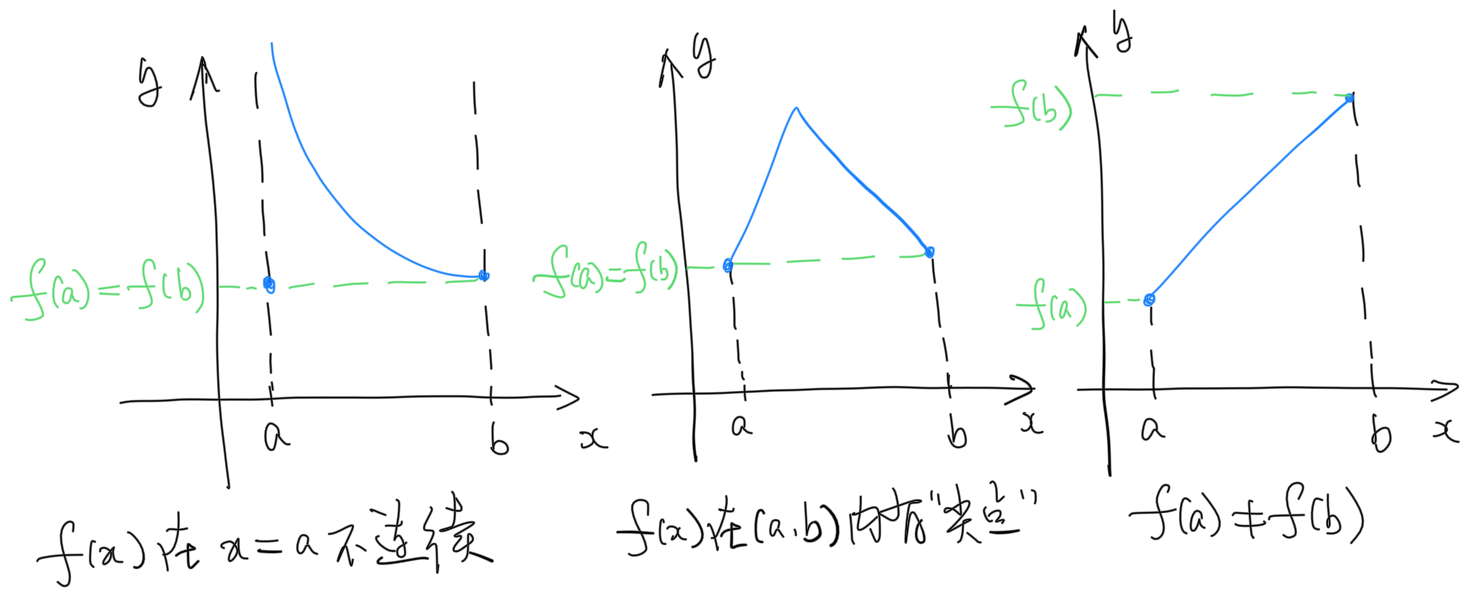
\includegraphics[width=0.8\textwidth]{./images/ch3/antiRolle.jpg}
\end{center}

{\bf 例:}证明:对函数$f(x)=(x-1)(x-2)(x-3)$,至少存在一点
$\xi\in(1,3)$,使得$f\,''(\xi)=0$。

[证]:$f(x)$是任意阶可导的,且在$[1,2],[2,3]$上均满足Rolle定理条件,
故必存在$\xi_1\in(0,1),\xi_2\in(2,3)$,使得
$$f'(\xi_1)=f'(\xi_2)=0.$$
进一步地,容易验证$f'(x)$在$[\xi_1,\xi_2]$上满足Rolle定理条件,
故必存在$\xi\in(\xi_1,\xi_2)$,使得$f''(\xi)=0$。
\hfill$\Box$

参照这个例题的证明思路,可以很容易地得到如下的推论:

\begin{thx}
	{\bf Rolle定理的高阶推广}:
	设$f(x)$在$[x_0,x_n]$上有$n-1$阶连续导函数,在$(x_0,x_n)$内
	$n$阶可导,且
	$$f(x_0)=f(x_1)=\ldots=f(x_n),\quad(x_0<x_1<\ldots<x_n),$$
	则存在$\xi\in(x_0,x_n)$,使得$f^{(n)}(\xi)=0$。
\end{thx}

利用Rolle定理证明可以证明一些有趣的结论,也可以构造出很多看似花样百出
的{\it 存在性问题}:

{\bf 例:}设$\df{a_0}{n+1}+\df{a_1}{n}+\ldots+a_n=0$,证明:方程
$$a_0x^n+a_1x^{n-1}+\ldots+a_n=0$$
在区间$(0,1)$内至少有一个根。

[提示]:令
$$F(x)=\df{a_0}{n+1}x^{n+1}+\df{a_1}{n}x^n+\ldots+a_nx$$

{\bf 例:}设$f(x)\in C[a,b]$,在$(a,b)$内可导,且$f(a)=f(b)=0$,证明:存在
$\xi\in(a,b)$,使得:
$$f'(\xi)+f(\xi)=0.$$

[提示]:$F(x)=f(x)e^x$

\begin{thx}
	辅助函数的构造可以从{\it 不定积分}(求导的逆运算)中获得一些启发
	\begin{itemize}
	  \setlength{\itemindent}{1cm}
	  \item $f(\xi)+\lambda f'(\xi)=0$:令$F(x)=e^{\lambda x}f(x)$
	  \item $f'(\xi)+f(\xi)g'(\xi)=0$: 令$F(x)=e^{\lambda g(x)}f(x)$
	  \item $nf(\xi)+xf'(\xi)=0$: 令$F(x)=x^nf(x)$ 
	  \item $f'(\xi)g(\xi)+f(\xi)g'(\xi)=0$:令$F(x)=f(x)g(x)$
	  \item $f'(x)g(x)-f(x)g'(x)=0$: 令$F(x)=\df{f(x)}{g(x)}$
	\end{itemize}
\end{thx}

\begin{shaded}

	{\bf 例}({\kaishu Darboux定理})设$f(x)$在$[a,b]$上可导,
	且$f\,'_+(a)f\,'_-(b)<0$,则存在$\xi\in(a,b)$,使得$f\,'(\xi)=0$。
	
	\begin{center}
		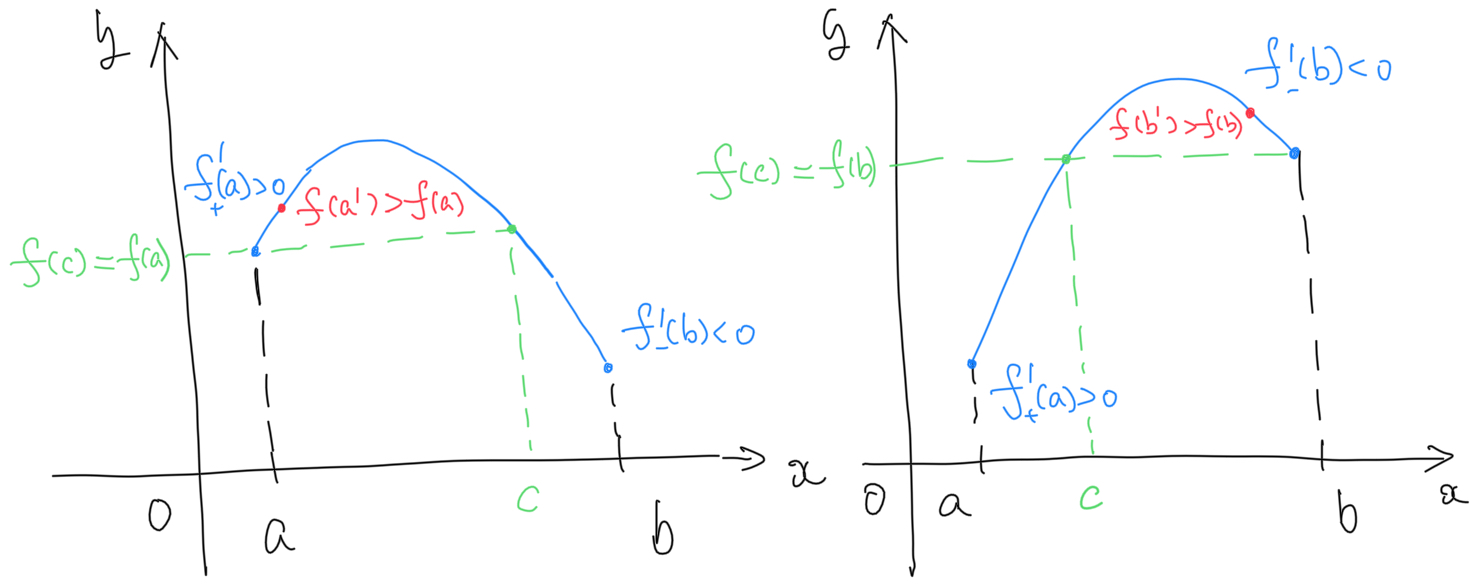
\includegraphics[width=0.8\textwidth]{./images/ch3/Darboux.jpg}
		
		\kaishu Darboux定理的证明思路
	\end{center}
	
	[证]:不妨设$f'_+(a)>0$,且$f(a)>f(b)$(如左图)。
	
	由$f'_+(a)>0$,也即$\limx{a^+}\df{f(x)-f(a)}{x-a}>0$,
	由极限的保号性,必存在某个$a'>a$,使得$\df{f(a')-f(a)}{a'-a}>0$,
	进而$f(a')>f(a)$。
	
	显然$f(x)$在$[a',b]$上连续,$f(a)\in(f(b),f(a'))$,故由介值定理,
	必存在$c\in(a',b)$,使得$f(c)=f(a)$。
	注意到$f(x)$在$[c,b]$上满足Rolle定理条件,故必存在$\xi\in(c,b)\subset(a,b)$,
	使得$f'(\xi)=0$。\hfill$\Box$
	
	Darboux定理说明{\it\b 导函数具有介值性},即可以证明:介于区间端点处的导数值之间的所有
	导数值,都可以在区间内部的某点上取到(请自行尝试证明)。
	介值性和连续性的关系一度是微积分理论中的难题,人们曾经猜想介值性和连续性是等价的,
	直到发现不连续的导函数(例如:$f(x)=x^2\sin\frac1x$的导函数在$x=0$不连续),
	并且通过Darboux定理验证了导函数的介值性,才发现这个猜想是错误的。
	
	采用与证明Darboux定理类似的方法,可以证明如下的结论:
	
	{\bf 例:}设$f(x)$在$[a,b]$上满足Rolle定理条件,
	且$f\,'_+(a)f\,'_-(b)>0$,则$f\,'(x)=0$在$(a,b)$内至少有两个根。
	
	\begin{center}
		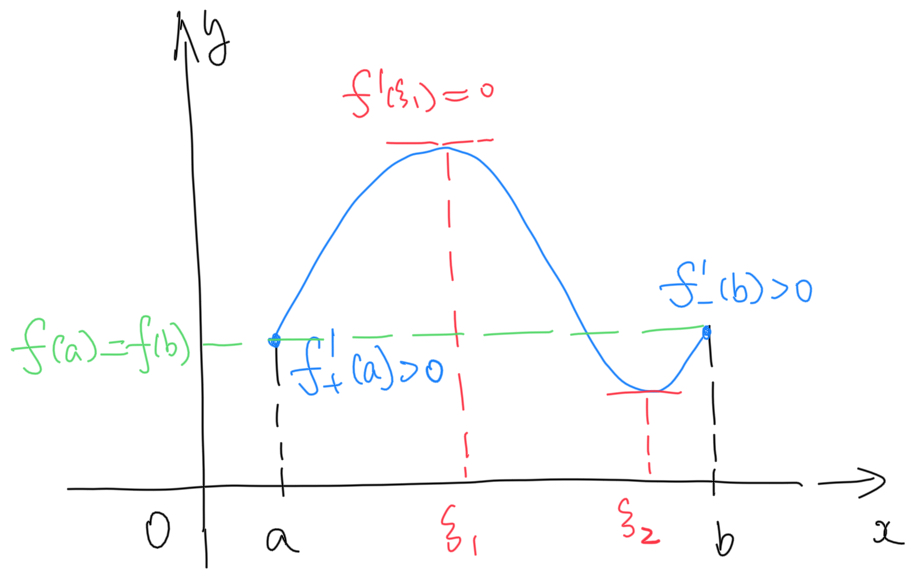
\includegraphics[width=0.5\textwidth]{./images/ch3/Darboux2.jpg}
		
		\it 示意图
	\end{center}
	
	[提示]:先利用Rolle定理证明存在$\xi_1$,再根据$f(\xi_1)$与$f(a)$的大小关系,
	采用与证明Darboux定理类似的方法证明$\xi_2$的存在。
\end{shaded}

\subsection{Lagrange中值定理}

下面这个定理据说实际上是由Cauchy证明的:

\begin{thx}
	{\bf Lagrange中值定理}:若函数$f(x)$满足:
	\begin{enumerate}[(1)]
	  \setlength{\itemindent}{1cm}
	  \item 在区间$[a,b]$上连续 
	  \item 在区间$(a,b)$内可导 
	\end{enumerate}
	则:存在$\xi\in(a,b)$,使得 
	$$f\,'(\xi)=\df{f(b)-f(a)}{b-a}.$$
\end{thx}

[提示]:结论即为\ps{\b 从结论出发构造辅助函数是证明中值问题的常用思路}
$$f'(\xi)(b-a)-[f(b)-f(a)]=0,$$
考虑
$$F'(x)=f'(x)(b-a)-[f(b)-f(a)],$$
则
$$F(x)=f(x)(b-a)-[f(b)-f(a)]x+C,$$
不妨令$C=0$,可以验证$F(b)=F(a)=bf(a)-af(b)$,再利用Rolle定理即可。

关于该证明的构造思路,有着非常生动形象的几何解释,具体请参见教材。从图示上看,
新构造的$F(x)$相当于是将原来的$f(x)$两端“拉平”(按比例平移)后得到的,
这种变换的一个重要特点是变换前后两个函数的连续性和可导性完全一致。

然而,从我们的分析过程来看,求解此类题目,完全不需要任何几何的直观,
可以直接从结论出发,通过求导的逆向过程(也就是{\it 不定积分})来构造出
所需的辅助函数。

Lagrange中值定理的结论有时也写作:
\begin{thx}
	{\bf Lagrange中值定理的另一种形式:}存在$(\theta\in(0,1))$,使得
	$$f(x+\Delta x)=f(x)+f'(x+\theta\Delta x)\Delta x.$$
\end{thx}

{\bf 例:}证明:
\begin{enumerate}[(1)]
  \setlength{\itemindent}{1cm}
  \item 导数恒为零的函数取值恒为常数。
  \item 导数恒大于零的函数严格单调递增。
\end{enumerate}

{\bf 例:}证明方程$x^5+x-1=0$只有唯一实根。

{\bf 例:}证明:$\df{\ln x-\ln x_1}{x-x_1}<\df 1{x_1},\quad (0<x_1<x)$

{\bf 例:}证明不等式:$\df{x}{1+x}<\ln(1+x)<x,\;x>0$

% {\bf 注:}在证明Eular常数
% $$\gamma=\limn\left(1+\df12+\ldots+\df1n-\ln n\right)$$
% 时,用到了这个不等式。

{\bf 例:}设$f(x)\in C[a,b]$,且$f(x)$在$(a,b)$内二阶可导,
连接函数曲线两端点的直线在$(a,b)$内至少与曲线存在一个交点,
则存在$\xi\in(a,b)$,使得$f\,''(\xi)=0$。

{\bf 思考:}{\b 若函数曲线的端点连线与函数曲线存在多个交点,能够得到什么结论?}

{\bf 例:}设$f(x)$在$[a,b]$上二阶可导,$f(a)=f(b)=0$,证明:对任意
$c\in(a,b)$,存在$\xi\in(a,b)$,使得
$$f(c)=\df{f\,''(\xi)}{2}(c-a)(c-b)$$

[提示]:设
$$F''(x)=f''(x)-\df{2f(c)}{(c-a)(c-b)},$$
则可得
$$F(x)=f(x)-\df{f(c)}{(c-a)(c-b)}x^2+C_1x+C_2,$$
其中$C_1,C_2$为常数。不妨令$C_1=C_2=0$,以下可以验证:
$$\df{F(c)-F(a)}{c-a}=\df{F(b)-F(c)}{b-c}
=-\df{f(c)}{(c-a)(c-b)}(a+b),$$
由Lagrange中值定理,存在$\xi_1\in(a,c),\xi_2\in(c,b)$,使得
$$F'(\xi_1)=F'(\xi_2)=-\df{f(c)}{(c-a)(c-b)}(a+b),$$
进而再由Rolle定理,存在$\xi\in(\xi_1,\xi_2)$,使得$F''(\xi)=0$,即证。

[注]:直接令辅助函数
$$F(x)=f(x)-\df{(x-a)(x-b)}{(c-a)(c-b)}f(c)$$
亦可,这个辅助函数的右半部分事实上是过$(a,0),(b,0),(c,f(c))$
三点的{\kaishu Lagrange插值多项式}!

\begin{shaded}
	\begin{tcolorbox}
		{\bf 过$n$个点$(x_i,f(x_i))(i=1,2,\ldots,n)$的Lagrange插值多项式}
		$$L_n(x)=\sum\limits_{i=1}^n\prod_{j=1,j\ne i}^{n}
		\df{x-x_j}{x_i-x_j}f(x_i)$$
	\end{tcolorbox}
	
	插值可以理解成利用一条曲线在给定的点之间“穿插”,而插值多项式就是用于穿插
	(连接)所有给定点的一个多项式函数。在工程应用中,对离散的观测数据进行建模,
	得到反映变化(运动)规律的函数曲线,从而对未来的变化(运动)趋势进行预测,
	是很常见的问题。
	
	{\bf 例:}过点$(0,0),(1,2),(2,-1),(3,-2)$的Lagrange插值多项式为
	$$L(x)=\df{x^3}6-8x^2+\df{41}6x$$
	
	\begin{center}
		\resizebox{!}{5cm}{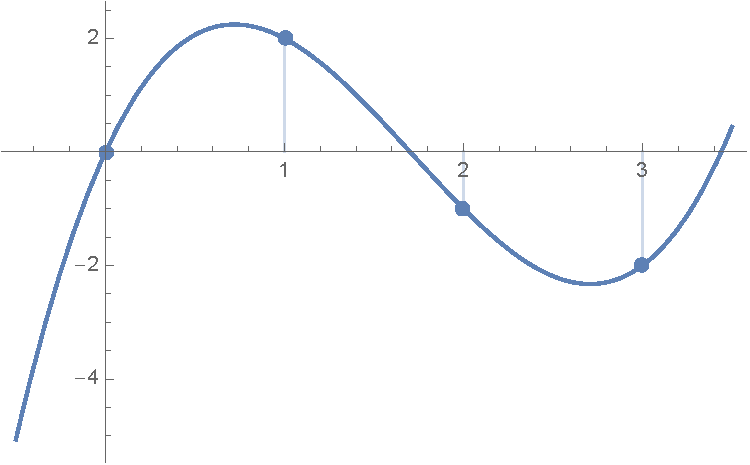
\includegraphics{./images/ch5/L4x.pdf}}
	\end{center}
	%% code of Mathematica 
	% f[x_] := 7/6*x^3 - 6 x^2 + 41/6*x;
	% CCurve = Plot[f[x], {x, -0.5, 3.5}];
	% DCurve = ListPlot[Table[{n, f[n]}, {n, 0, 3}], Filling -> Axis];
	% Show[CCurve, DCurve]
\end{shaded}

{\bf 例:}证明:$\df{e^a-e^b}{b-a}<\df{e^a+e^b}2,\;(a\ne b)$

分析:不妨$a<b$,令$f(x)=\df{e^a+e^x}2-\df{e^a-e^x}{b-a}$

{\bf 例:}$f(x)$在$[0,1]$上二阶可导,$f(0)=0,f(1)=1$,$f''(0)<0$,则
$\df{f(x)}x$在$(0,1]$上严格单调递减

{\bf 例:}$y=f(x)\in C^2(-1,1)$,$f''(x)\ne 0$,则:
\begin{enumerate}[1)]
  \setlength{\itemindent}{1cm}
  \item 对于任意$x\in(-1,1),x\ne 0$,存在唯一的$\theta(x)\in(0,1)$,使得
  $f(x)=f(0)+xf'(\theta(x)x)$成立
  \item $\limx{0}\theta(x)=\df12$
\end{enumerate}

分析:1)Lagrange中值定理,若$\theta(x)$不唯一,则与$f''(x)\ne 0$矛盾;

2)
$$\df{f'(\theta(x)x)-f'(0)}{x}=\df{f(x)-f(0)-xf'(0)}{x^2}\to\df12f''(0),(x\to0)$$
$$\df{f'(\theta(x)x)-f'(0)}{x}=f''(0)\limx{0}\theta(x)$$

\subsection{Cauchy中值定理}

\begin{thx}
	{\bf Cauchy中值定理}:若函数$f(x),\varphi(x)$满足: 
	\begin{enumerate}[(1)]
	  \setlength{\itemindent}{1cm}
	  \item 在$[a,b]$上连续 
	  \item 在$(a,b)$内可导,且$\varphi'(x)\ne 0$ 
	\end{enumerate}
	则:存在$\xi\in(a,b)$, 使得
	$$\df{f(b)-f(a)}{\varphi(b)-\varphi(a)}=\df{f'(\xi)}{\varphi'(\xi)}$$
\end{thx}

[提示]:结论即为
$$[f(b)-f(a)]\varphi'(\xi)-[\varphi(b)-\varphi(a)]f'(\xi)=0,$$
因此考虑
$$F'(x)=[f(b)-f(a)]\varphi'(x)-[\varphi(b)-\varphi(a)]f'(x),$$
从而
$$F(x)=[f(b)-f(a)]\varphi(x)-[\varphi(b)-\varphi(a)]f(x)+C.$$
不妨令$C=0$,可以验证$F(b)=F(a)$,利用Rolle定理即可。

这个证明思路延续了我们此前证明很多中值问题所使用的方法,与教材上的方法存在
比较明显的差异,但从解题的角度来看,更具普遍的可操作性。

{\bf 注:}Cauchy中值定理可视为{\it 参数化}的Lagrange中值定理,即:
由$\varphi'(x)\ne 0$可知,$\varphi(x)$为单调(可逆)函数,从而设
$A=\varphi(a),B=\varphi(b)$,故由Lagrange中值定理,存在$\xi\in(a,b)$,
也即$C=\varphi(\xi)$介于$A,B$之间,使得
$$\df{f(b)-f(a)}{\varphi(b)-\varphi(a)}
=\df{f(\varphi^{-1}(B))-f(\varphi^{-1}(A))}{B-A}
=[f(\varphi^{-1}(x))]'_{x=\xi}=\df{f'(\xi)}{\varphi'(\xi)}.$$

通过对结论适当变形整理,以上结论都可以使用Rolle定理证明。

\begin{ext}
	{\bf 课后作业}
	
	\begin{enumerate}
	  \item 设$0<a<b$,$f(x)$在$[a,b]$上连续,在$(a,b)$内可导,证明:
		\begin{enumerate}[(1)]
% 		  \setlength{\itemindent}{1cm}
		  \item 存在$\xi\in(a,b)$,使得:
			$$f(b)-f(a)=\ln\df ba\cdot \xi f\,'(\xi)$$
		  \item 存在$\eta\in(a,b)$,使得:
		    $$2\eta[f(b)-f(a)]=(b^2-a^2)f\,'(\eta)$$
		  \item 存在$x_1,x_2,x_3\in(a,b)$,使得
			$$f\,'(x_1)=(b+a)\df{f\,'(x_2)}{2x_2}=(a^2+ab+b^2)
			\df{f\,'(x_3)}{3x_3^2}$$ 
		  \item 若$f\,'(x)\ne 0$,则存在$\xi,\eta\in(a,b)$,使得
			$$\df{f'(\xi)}{f'(\eta)}=\df{e^b-e^a}{b-a}e^{-\eta}$$
		  \item 存在$c\in(a,b)$,使得
			$$\df{1}{a-b}\left|\begin{array}{cc}
			a & b\\ f(a) & f(b)
			\end{array}\right|=f(c)-cf'(c).$$
		  \item (选作)若$f(a)=0$,则存在$\mu\in(a,b)$,使得
		  $$f'(\mu)=\df{a}{a+b-2\mu}f(\mu).$$
		\end{enumerate}
	  \item (选作)$f(x)\in C^1[a,b]$,$f(a)=f(b)=0$,$f'_+(a)f'_-(b)>0$,
	  证明:$f(x)$在$(a,b)$内至少有一个零点。
	  (利用极限的保号性,说明在$a,b$附近各有一点,两点函数值反号,然后利用介值定理)
	  \item 证明:$(x^2-1)\ln x\geq(x-1)^2,(x>0)$。
	  \item $e<a<b<e^2$,证明:$\ln^2b-\ln^2a>\df4{e^2}(b-a)$
% 		分析:$f(x)=\ln^2x$,由Lagrange中值定理,存在$\xi\in(a,b)$,
% 		$$\df{\ln^2b-\ln^2a}{b-a}=\df{2\ln\xi}{\xi},$$
% 		再证明$\df{\ln\xi}{\xi}>\df2{e^2},\xi\in(a,b)\in(e,e^2)$
	  \item (选作)$f(x)$在$x>0$二阶可导,$f''(x)>0$,令$u_n=f(n)\;
	  (n\in\mathbb{Z}_+)$,证明:若$u_1<u_2$,则$\{u_n\}$必发散;
	  问:若$u_1>u_2$,$\{u_n\}$是否必收敛?(若正确,证明之;否则给出反例。)
% 	  分析:$u_1<u_2$,则$\exists\xi\in(1,2)$,$f'(\xi)>0$,
% 		又$x>\xi$时,$f'(x)>f'(\xi)$,故
% 		$$f(x)>f(\xi)+f'(\xi)(x-\xi)\to+\infty\;(x\to+\infty)$$
	\end{enumerate}
\end{ext}

\section{L'Hospital法则}

在第一章的“无穷小比较”一节,我们曾讨论过一些不定式极限,这类极限的特点是
从其自身的构造特定,无法直接看出极限的结果,因此成为极限计算问题中一类
颇有难度的问题。和用无穷小代换的方法计算极限相比,L'Hospital法则在用法
上显得更为简单,应用的范围也非常广泛,因此可以被称为是“最受欢迎”的的
一类极限计算方法。

常见的不定式(型)极限包括如下一些类型:\ps{$0,1,\infty$在此均表示一种趋势,而不是具体的值}
$$\bm{\df{0}{0}}, \quad \bm{\df{\infty}{\infty}}, \quad
\bm{1^{\infty}}, \quad \bm{0\cdot\infty}, \quad
\bm{\infty-\infty}, \quad \bm{\infty^0}, \bm{\quad 0^0}$$
\begin{center}
	\resizebox{!}{3.5cm}{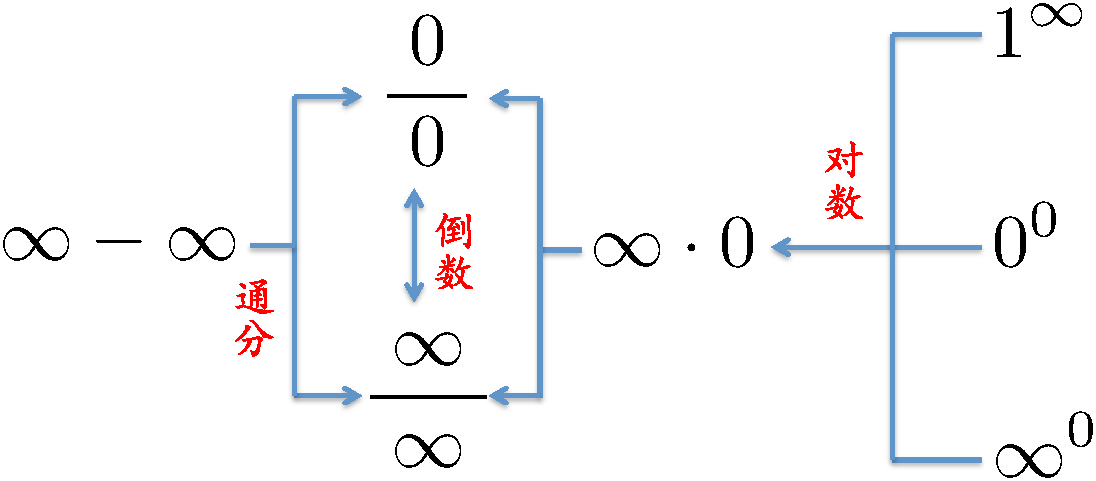
\includegraphics{./images/ch5/lim00.pdf}}
\end{center}
通过与各种函数运算相结合,它们之间可以实现互相的转化,因此和此前类似,在此
我们只讨论前两种情形的极限计算方法即可。

% {\bf 举例:}
% \begin{enumerate}[(1)]
%   \setlength{\itemindent}{1cm}
%   \item $\limx{0}\df{x-\sin x}{x}$ 
%   \item $\limx{+\infty}\df{\ln x}{x}$ 
%   \item $\limx{1}(1-x^2)\tan\df{\pi}2x$ 
%   \item $\limx{0}(x^2+2^x)^{1/x}$
% \end{enumerate}

L'Hospital是一个“著名”的数学爱好者,他为John Bernoulli提供赞助,并获得
对方一些最新的研究结果。以下的求极限法则最初由后者发现,而由前者发表并命名,
Bernoulli后来为此感到非常后悔,曾想要回这个本属于自己的定理。

\begin{thx}
	{\bf 计算$\df00$型不定式极限的L'Hospital法则(I):}设
	\begin{enumerate}[(1)]
	  \item $\limx{a}f(x)=\limx{a}F(x)=0$;
	  \item $f(x)$和$F(x)$在$a$的某去心邻域内可导,且$F'(x)\ne0$;
	  \item $\limx{a}\df{f'(x)}{F'(x)}$存在,或为无穷大,
	\end{enumerate}
	则
	$$\limx{a}\df{f(x)}{F(x)}=\limx{a}\df{f'(x)}{F'(x)}.$$
\end{thx}

[证]:由条件(1),不妨设$f(a)=F(a)=0$,任取$x$为条件(2)所述$a$的去心邻域内一点,
则$f(x)$和$F(x)$在$a$到$x$的区间内满足Cauchy中值定理条件,从而
存在$\xi$介于$a$和$x$之间,使得
$$\df{f(x)}{F(x)}=\df{f(x)-f(a)}{F(x)-F(a)}
=\df{f'(\xi)}{F'(\xi)},$$
在该式两端{\b 令$x\to a$,由$\xi$的特性可知,必有$\xi\to a$},进而由
条件(3)即证。\hfill$\Box$

以上结论可以直接推广到$\infty/\infty$不定式的情形,事实上:
若条件(1)改为$\limx{a}f(x)=\limx{a}F(x)=+\infty$,则
$\limx{a}\df1{f(x)}=\limx{a}\df1{F(x)}=0$;由条件(2)
可得$\df1{f(x)}$和$\df1{F(x)}$均可导,且$[1/F(x)]'\ne 0$;
条件(3)不变,对$\df1{f(x)}$和$\df1{F(x)}$直接使用以上定理的结论,可得
$$
	\limx{a}\df{f(x)}{F(x)}
	=\limx{a}\df{1/F(x)}{1/f(x)}
	=\limx{a}\df{[1/F(x)]'}{[1/f(x)]'}
	=\limx{a}\df{F'(x)}{f'(x)}\limx{a}\df{f^2(x)}{F^2(x)},
$$
稍加整理,即得结论。关于这个结论有一个形象的解释:两个物体都飞向无穷远处,
他们所经历的路程之比最终取决于他们的速度之比。

在使用L'Hospital法则时,特别需要注意的是
{\b 由$\limx{\Delta}\df{f'(x)}{g'(x)}=A$可以推出
$\limx{\Delta}\df{f(x)}{g(x)}=A$,但反之不然。}反例如下:
$\limx{+\infty}\df{x+\sin x}x=1$,
但$\limx{+\infty}(1+\cos x)$不存在!

最后,对于$x$趋于无穷时的极限,也有类似的结论,证明在此略过。

\begin{thx}
	{\bf 计算$\df00$型不定式极限的L'Hospital法则(II):}设
	\begin{enumerate}[(1)]
	  \item $\limx{\infty}f(x)=\limx{\infty}F(x)=0$;
	  \item $f(x)$和$F(x)$在当$x$充分大时可导,且$F'(x)\ne0$;
	  \item $\limx{\infty}\df{f'(x)}{F'(x)}$存在,或为无穷大,
	\end{enumerate}
	则
	$$\limx{\infty}\df{f(x)}{F(x)}=\limx{\infty}\df{f'(x)}{F'(x)}.$$
\end{thx}

{\bf 例:}计算如下极限
\begin{enumerate}[(1)]
  \setlength{\itemindent}{1cm}
  \item $\limx{0}\df{x-\sin x}{x^3}$ 
  \item $\limx{0}\df{e^x-e^{-x}-2x}{\tan^3x}$ 
%   \item $\limx{0}\df{(1+x)^{1/x}-e}{x}$ 
  \item $\limx{+\infty}\df{x^n}{e^{\lambda
  x}}(n\in\mathbb{N},\lambda>0)$ 
  \item $\limx{+\infty}\df{\ln x}{x^\alpha}(\alpha>0)$ 
  \item $\limx{\infty}\df{x+\sin x}{x+\cos x}$
%   \item $\limx{1}(1-x^2)\tan\df{\pi}{2}x$ 
%   \item $\limx{0}\left(\df 1{x^2}-\df 1{x\tan x}\right)$ 
  \item $\limx{0^+}x^x$
%   \item $\limx{0}(x^2+2^x)^{1/x}$ 
%   \item $\limx{0}\left(\cot x-\df 1x\right)$ 
  \item $\limn\sqrt[n]n$
  \item $\limx0\left(\df{\sin x}x\right)^{\frac1{1-\cos x}}=-\df13$
\end{enumerate}

{\bf 注:}在使用L'Hospital法则时,一个重要的原则是及时化简,同时注意和其他
计算极限的方法(例如无穷小代换)结合使用,避免对函数反复求导,导致分子分母的表达式
越来越复杂,无法化简得到结果。

{\b{\bf 讨论:}设$f(x)$在$x_0$附近存在二阶连续导函数,则
$$\lim\limits_{h\to 0}\df{f(x_0+h)+f(x_0-h)-2f(x_0)}{h^2}=f\,''(x_0).$$
若条件减弱为“$f(x)$在$x=x_0$处二阶可导”,结论是否仍然成立?\ps{难点!}

[答]:成立,如果条件是$f(x)$在$x_0$附近存在二阶连续导函数,可以如下进行推导,
\begin{align}
	\lim\limits_{h\to 0}&\df{f(x_0+h)+f(x_0-h)-2f(x_0)}{h^2}
	=\lim\limits_{h\to 0}\df{f'(x_0+h)-f'(x_0-h)}{2h}\notag\\
	&=\lim\limits_{h\to 0}\df{f''(x_0+h)+f''(x_0-h)}{2}
	=f''(0)\notag
\end{align}
但如果条件减弱为$f(x)$在$x=x_0$处二阶可导,这样的推导就是不对的。
其中的错误在于,此时不能保证$f(x)$在$x_0$以外的点(例如$x_0\pm h$)
处存在二阶导数,更谈不上二阶导数连续,因此最后的两个等号都是不成立的!

事实上,正确的推导应该是
\begin{align}
	\lim\limits_{h\to 0}&\df{f(x_0+h)+f(x_0-h)-2f(x_0)}{h^2}
	=\lim\limits_{h\to 0}\df{f'(x_0+h)-f'(x_0-h)}{2h}\notag\\
	&=\df12\lim\limits_{h\to 0}\df{f'(x_0+h)-f'(x_0)}{h}
	+\df12\lim\limits_{h\to 0}\df{f'(x_0-h)-f'(x_0)}{-h}
	=f''(0)\notag
\end{align}
其中最后一个等号只用到了二阶导数的定义。}

{\bf :}设$f(x)$在$x=a$处二阶可导,且$f'(a)\ne0$,证明:
$$\limx{a}\left[\df1{f(x)-f(a)}-\df1{(x-a)f'(a)}\right]
=-\df12\df{f''(a)}{[f'(a)]^2}.$$

在L'Hospital法则的证明中,“令$x\to a$时,由于$\xi$介于$x$和$a$之间,进而
有$\xi\to a$”,这是一个非常有用的技巧,利用这一技巧,可以证明类似如下的结论:

{\bf 例:}设$\limx{+\infty}f(x)$和$\limx{+\infty}f\,'(x)$均存在,证明:
$$\limx{+\infty}f\,'(x)=0.$$

[证]:由Lagrange中值定理,对任意$x\in\mathbb{R}$,存在$\xi\in[x,x+1]$,满足
$$f(x+1)-f(x)=f'(\xi),$$
注意到{\b$x\to+\infty\Leftrightarrow\xi\to+\infty$},
$\limx{+\infty}f(x+1)=\limx{+\infty}f(x)$,故
$$0=\limx{+\infty}[f(x+1)-f(x)]=\limx{+\infty}f'(\xi)
=\lim\limits_{\xi\to+\infty}f'(\xi)=\limx{+\infty}f'(x)$$
即证。

{\bf 例:}设$f(x)$在$U(x_0)$内连续,在$U^0(x_0)$内可导,
且$\limx{x_0}f\,'(x)=l$,则$$f\,'(x_0)=l.$$

[证]:由Lagrange中值定理,对任意$\Delta x\in\mathbb{R}$,存在
$\xi\in[x_0,x_0+\Delta x]$,使得
$$\df{f(x_0+\Delta x)-f(x_0)}{\Delta x}=f'(\xi),$$
注意到{\b$\Delta x\to 0\Leftrightarrow\xi\to0$},故
$$f'(x_0)=\lim\limits_{\Delta x\to 0}\df{f(x_0+\Delta x)-f(x_0)}{x_0}
=\lim\limits_{\Delta x\to 0}f'(\xi)=\lim\limits_{\xi\to 0}f'(\xi)=l,$$
即证。

{\bf 例:}
设$f(0)=1$,且
$$\limx{0}\df{\ln(1-x)+f(x)\sin x}{e^{x^2}-1}=0,$$
证明:$f(x)$在$x=0$处可导,求$f\,'(0)$。

\begin{ext}
	{\bf 课后作业}
	
	\begin{enumerate}
	  \item 计算如下极限
		\begin{enumerate}[(1)]
% 		  \setlength{\itemindent}{1cm}
		  \item $\limx{0^+}\df{\ln\tan 7x}{\ln\sin 3x}$
		  \item $\limx{+\infty}\df{\ln\left(1+\df1n\right)}{\arctan x}$
		  \item $\limx{0^+}x^{\sin x}$
		  \item $\limx{\infty}x^2e^{\frac1{x^2}}$
		  \item $\limx{\infty}\df{x^2-\cos x}{x^2+\sin x}$
		  \item $\limx{0}\df{x^2-\sin x}{x^2+\cos x}$
		  \item $\limx{0}\df{\ln(1+x^2)}{\sec x-\cos x}$
  		  \item $\limx{0}\df{(1+x)^{1/x}-e}{x}$ 
   		  \item $\limx{1}(1-x^2)\tan\df{\pi}{2}x$ 
  		  \item $\limx{0}\left(\df 1{x^2}-\df 1{x\tan x}\right)$ 
  		  \item $\limx{0}(x^2+2^x)^{1/x}$ 
  		  \item $\limx0\df{e^{\tan x}-e^x}{\tan x-x}$
  		  \item $\limx{0}\left(\cot x-\df 1x\right)$ 
  		  \item $\limx{\infty}\left[\df1n\left(a_1^{\frac1x}+a_2^{\frac1x}
  		  +\ldots+a_n^{\frac1x}\right)\right]^{nx}$,其中$a_1,a_2,\ldots,a_n>0$
		\end{enumerate}
	  \item 讨论函数
	  $$f(x)=\left\{\begin{array}{ll}
	  	\left[\df{(1+x)^{\frac1x}}e\right]^{\frac1x},& x>0,\\
	  	e^{-\frac12},& x\leq 0.
	  \end{array}\right.$$
	  在$x=0$处的连续性。
	\end{enumerate}
\end{ext}

\section{Taylor公式}

Taylor公式直观地说是对给定函数的一种{\it 多项式逼近},也即用一个多项式函数
近似地表示某个给定的函数。相对于微分所体现的“以直代曲”,这种逼近方式可以称为
“以曲代曲”,不难想到,由于多项式函数的类型比线性函数(事实上就是$1$阶的多项式)
更加丰富,这样的逼近效果应该会更好。下面,我们首先从“以曲代曲”
的角度引入Taylor多项式的概念,然后分析其逼近的效果,最后给出Taylor公式
的有关应用。可以说,Taylor公式是整个微分学的“制高点”,其中蕴含了微分学中
的众多结论,或者说,微分学中的众多结论其实都只是它的推论而已。

“以曲代曲”的核心是所谓的{\it $n$阶相切}:

\begin{thx}
	$P_n(x)$称为{\bf $f(x)$在点$x_0$处的$n$阶Taylor多项式},若
	\begin{itemize}
% 	  \setlength{\itemindent}{1cm}
	  \item $P_n(x)$是$n$次多项式,形如:$\sum\limits_{k=0}^na_k(x-x_0)^k$;
	  \item $y=P_n(x)$在$x_0$处与$y=f(x)$处至少{\bf $n$阶相切},即
	  对任意$k=0,1,2,\ldots,n$,有
	  $$P^{(k)}_n(x_0)=f^{(k)}(x_0).$$
	%   \begin{enumerate}[(1)]
	%     \item $P_n(x_0)=f(x_0)$
	%     \item $P'_n(x_0)=f'(x_0)$
	%     \item $P''_n(x_0)=f''(x_0)$
	%     \item \ldots
	%     \item $P^{(n)}_n(x_0)=f^{(n)}(x_0)$
	%   \end{enumerate} 
	\end{itemize}
	特别地,若$x_0=0$,$P_n(x)$称为{\bf $f(x)$的$n$阶Maclaurin多项式}
\end{thx}

根据以上定义,可设
$$P_n(x)=a_0+a_1(x-x_0)+a_2(x-x_0)^2+\ldots+a_n(x-x_0)^n,$$
对其两边逐次求导(直至$n$阶导数),然后令$x=x_0$,不难得到
\begin{align*}
	P_n(x_0)&=a_0,\\
	P'_n(x_0)&=a_1,\\
	P''_n(x_0)&=2a_2,\\
	P^{(3)}_n(x_0)&=3!a_3,\\
	\ldots&\ldots\\
	P^{(n)}_n(x_0)&=n!a_n.\\
\end{align*}
利用以上定义中的第二个条件,解得
$$a_k=\df{f^{(n)}(x_0)}{k!},\;k=0,1,2,\ldots,n.$$
至此就得到了
\begin{thx}
	{\bf $f(x)$在点$x_0$处的$n$阶Taylor多项式:}
	$$P_n(x)=\sum\limits_{k=0}^n\df{f^{\,(k)}(x_0)}{k!}(x-x_0)^k$$
\end{thx}
这个公式说明,给定$f(x)$、$x_0$和$n$,$P_n(x)$是唯一确定的。更直观地说,
{\it\b 要在给定点处,按照指定的(相切)阶数,近似表示给定的函数,
只有唯一的一个多项式可以满足条件}。

{\bf 例:}求下列函数的Maclaurin多项式
\begin{enumerate}[(1)]
  \setlength{\itemindent}{1cm}
  \item $f(x)=e^x$ 
  $${P_n(x)=1+x+\df{x^2}{2!}+\ldots+\df{x^n}{n!}}$$ 
  \item $f(x)=\cos x$ 
  $${P_{2m}(x)=1-\df{x^2}{2!}+\df{x^4}{4!}-\ldots+(-1)^m\cdot\df{x^{2m}}{(2m)!}}$$
\end{enumerate}

\subsection{误差估计}

有了Taylor多项式,接下来需要确认它是否是一个好的逼近。为此,我们首先给出余项和
Taylor公式的概念。

\begin{thx}
	\begin{itemize}
% 	  \setlength{\itemindent}{1cm}
	  \item {\bf 余项:}
	  $$R_n(x)=|f(x)-P_n(x)|$$ 
	  \item {\bf 带Peano余项的$n$阶Taylor公式:}
	  $$f(x)=P_n(x)+\circ[(x-x_0)^n]$$
	\end{itemize}
\end{thx}

可以看到Taylor公式由Taylor多项式和余项两个部分构成,今后如果允许使用“{\it 无穷次}”
的多项式(也就是{\it 幂级数}),则可以进一步得到所谓的{\kaishu Taylor级数}。


下面的定理说明多项式逼近是一种{\it 有效}的逼近,其在给定的点附近与给定函数的误差,
是自变量改变量的高次幂(取决于展开的阶数)一个高阶无穷小。

\begin{thx}
	{\bf Taylor公式的误差:}设函数$f(x)$在$x_0$处$n$阶可导,$P(x)$是$f(x)$在点$x_0$处
	的$n$阶Taylor多项式,则当$x\to x_0$时
	$${|f(x)-P_n(x)|=\circ[(x-x_0)^n]}$$
\end{thx}

需要特点指出一点,Taylor公式的{\b 阶数是多少,关键看余项!}例如$\sin x$的7阶和8阶Maclaurin公式分别为
$$\sin x=x-\df{x^3}{3!}+\df{x^5}{5!}-\df{x^7}{7!}+{\b\circ(x^7)},$$
$$\sin x=x-\df{x^3}{3!}+\df{x^5}{5!}-\df{x^7}{7!}+{\b\circ(x^8)}.$$

高阶无穷小形式的余项从理论意义上确保了Taylor多项式的逼近效果,但对于需要具体估计
逼近误差的场合,还是不够的,因此就有了所谓的{\kaishu Lagrange余项},对应的
Taylor公式也称为Taylor中值定理:

\begin{thx}
	{\bf Taylor中值定理:}设$f(x)$在$x_0$的某邻域内$n+1$阶可导,
	对该邻域内任一点$x$,存在介于$x_0$和$x$之间的一点$\xi$,满足
	$$f(x)=P_n(x)+\df{f^{(n+1)}(\xi)}{\,(n+1)!}(x-x_0)^{n+1}$$
\end{thx}

上式称为{\bf 带Lagrange余项的$n$阶Taylor公式},有时也写为
$${\b f(x_0+h)=P_n(x_0+h)+\df{f^{\,(n+1)}(x_0+\theta
h)}{(n+1)!}h^{n+1},(0<\theta<1)}$$
不难看出,Taylor中值定理是对Lagrange中值定理的推广。

[证]:
先考虑$x>x_0$的情况,其余情况可以类似地证明。注意到$P^{(n+1)}(x)=0$,
$f^{(k)}(x_0)=P^{(k)}_n(x_0),k=0,1,2,\ldots,n$,
反复利用Cauchy中值定理,存在$x_0<\xi<\xi_n<\xi_{n-1}
<\ldots<\xi_2<\xi_1<x$,使得
\begin{align}
	\df{f(x)-P_n(x)}{(x-x_0)^{n+1}}
	&=\df{f'(\xi_1)-P'_n(\xi_2)}{(n+1)(\xi_1-x_0)^{n}}
	=\df{f''(\xi_2)-P''_n(\xi_2)}{(n+1)n(\xi_2-x_0)^{n-1}}\notag\\
	&=\ldots=\df{f^{(n)}(\xi_n)-P^{(n)}_n(\xi_n)}{(n+1)!(\xi_n-x_0)}
	=\df{f^{(n+1)}(\xi)}{(n+1)!}\notag
\end{align}
即证。\hfill$\Box$

利用以上定理,立即可以得到如下推论:
\begin{thx}
	{\bf Taylor公式的误差估计:}若存在常数$C>0$,使当$x\in(a,b)$时,恒有
	$$|f^{\,(n+1)}(x)|\leq C,\;n=0,1,2,\ldots$$
	则
	$$\limn [f(x)-P_n(x)]=0.$$
\end{thx}
该推论告诉我们,{\it 在一定条件下}(各阶导数有界),Taylor多项式的次数越高,逼近精度就越高。

\begin{shaded}
	{\bf Taylor公式的适用条件}
	
	以下内容主要引自《数学桥》P92。
	
	除了要求被展开的函数应该具有高阶导数之外,在运用Taylor公式的时候,有一个
	条件特别我们需要注意。如果所讨论的函数的导数值增加得太快的话,这个结论就
	不成立了,因为我们无法让给定点附近的各阶导数都被某个确定值所界定。
	例如,下面的函数
	$$f(x)=\left\{\begin{array}{ll}
		\exp\left(-\df1{x^2}\right),&x\ne 0;\\
		0,& x=0.
	\end{array}\right.$$
	\begin{center}
		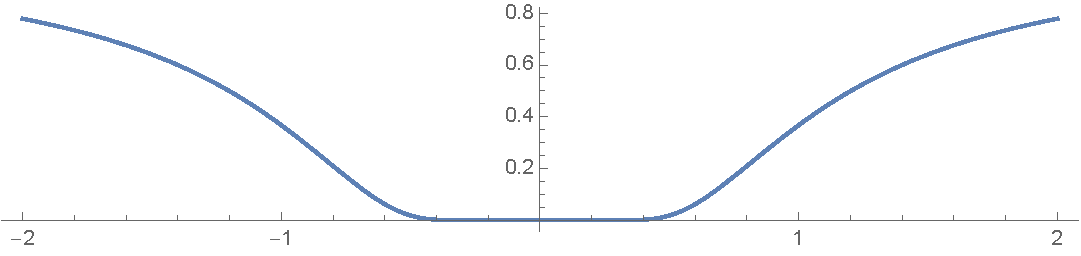
\includegraphics[width=0.6\textwidth]{./images/ch3/e-1x2.pdf}
	\end{center}
	通过计算,不难发现,对任意$n\in\mathbb{Z}^+$,均有
	$$f^{(n)}(0)=0.$$
	因此,$f(x)$在$x=0$处的Taylor公式就是
	$$f(x)=\sum\limits_{k=0}^n\df{0}{k!}x^k+\circ(x^n)
	=0+\circ(x^n).$$
	(更进一步说,$f(x)$的Taylor级数应该表示为$f(x)=0$。)
	这显然和原函数存在较大“出入”,问题出在哪里呢?
	
	问题在于$f(x)$的$n$阶导函数都包含如下的一部分
	$$\df{2^n}{x^{2n}}\exp\df1{-x^2}.$$
	对于任意给定的实数$C$,只要$|x|<1$,当$n$充分大时,该值总会超过$C$。
	由于这个原因,我们无法把原点任何邻域内的所有导数值都限定在一定的范围内,
	这意味着前面关于Taylor公式误差估计的结论不再有效,换言之,此时的
	Taylor多项式已经不是给定函数的一个有效逼近了。
\end{shaded}

\begin{thx}
	{\bf 一些常用的Maclaurin公式}
	\begin{enumerate}[(1)]
% 	  \setlength{\itemindent}{1cm}
	  \item $e^x =\sum\limits_{k=0}^n\df{x^k}{k!}
	  +\df{e^{\theta x}}{(n+1)!}x^{n+1}\;
	  (0<\theta<1,x\in\mathbb{R})$
	  \item $\sin x
	  =\sum\limits_{k=1}^m(-1)^{k-1}\df{x^{2k-1}}{(2k-1)!} 
	  +(-1)^m\df{\cos\theta x}{(2m+1)!}x^{2m+1}\;
	  (0<\theta<1,x\in\mathbb{R})$
	  \item $\cos x= \sum\limits_{k=0}^m(-1)^{k}\df{x^{2k}}{(2k)!}
	  +(-1)^{m+1}\df{\sin\theta
	  x}{(2m+2)!}x^{2m+2}\; (0<\theta<1,x\in\mathbb{R})$
	  \item
	  $\ln(1+x) =\sum\limits_{k=1}^n(-1)^{k-1}\df{x^k}{k}
	  +\df{(-1)^nx^{n+1}}{(n+1)(1+\theta
	  x)^{n+1}}\; (0<\theta<1,x>-1)$
	  \item
	  $(1+x)^\alpha =\sum\limits_{k=0}^n
	  \df{\alpha(\alpha-1)\ldots(\alpha-k+1)}{k!}x^k$

		\hspace{2cm}$+\df{\alpha(\alpha-1)\ldots(\alpha-n)}{(n+1)!}\df{x^{n+1}}{(1+\theta
		x)^{n+1-\alpha}}\quad (0<\theta<1,x\ne -1)$
	\end{enumerate}
\end{thx}

\begin{shaded}
	{\bf Taylor公式:等价无穷小的“宝库”}
	
	从Taylor公式出发,可以很容易地得到一些等价无穷小,例如,由
	$$\sin x=x-\df{x^3}{3!}+\df{x^5}{5!}-\df{x^7}{7!}+
	\ldots+(-1)^n\df{x^{2n+1}}{(2n+1)!}+\circ(x^{2n+1}).$$
	两边同时除以$x$,再令$x\to 0$,可得
	\begin{align*}
		\limx{0}\df{\sin x}x&=1+\limx{0}\df1x\left[-\df{x^3}{3!}+
		\df{x^5}{5!}-\df{x^7}{7!}+ 
		\ldots+(-1)^n\df{x^{2n+1}}{(2n+1)!}+\circ(x^{2n+1})\right]\\
		&=1+\limx{0}\left[-\df{x^2}{3!}+
		\df{x^4}{5!}-\df{x^6}{7!}+ 
		\ldots+(-1)^n\df{x^{2n}}{(2n+1)!}+\circ(x^{2n})\right]=1,
	\end{align*}
	故$x\to 0$时,
	$$\sin x\sim x.$$
	
	类似地,注意到
	$$\sin x-x=-\df{x^3}{3!}+\df{x^5}{5!}-\df{x^7}{7!}+
	\ldots+(-1)^n\df{x^{2n+1}}{(2n+1)!}+\circ(x^{2n+1}).$$
	两边同时除以$x^3$,再令$x\to 0$,可得
	\begin{align*}
		\limx0\df{\sin x-x}{x^3}
		&=-\df1{3!}+\limx0\df1{x^3}\left[\df{x^5}{5!}-\df{x^7}{7!}+ 
		\ldots+(-1)^n\df{x^{2n+1}}{(2n+1)!}+\circ(x^{2n+1})\right]\\
		&=-\df16+\limx0\left[\df{x^2}{5!}-\df{x^4}{7!}+ 
		\ldots+(-1)^n\df{x^{2n-2}}{(2n+1)!}+\circ(x^{2n-2})\right]
		=-\df16.
	\end{align*}
	由此可知,当$x\to 0$时,
	$$\sin x-x\sim -\df16x^3.$$
	
	依此类推,从$\sin x$的Taylor公式中可以得到许许多多的等价无穷小关系(当$x\to 0$时):
% 	\begin{tcolorbox}[breakable]
		\begin{align*}
			\sin x&\sim  x\\
			\sin x-x&\sim  -\df16x^3\\
			\sin x-x+\df{x^3}{3!} & \sim  \df{x^5}{5!}\\
			\sin x-x+\df{x^3}{3!}+\df{x^5}{5!} & \sim  -\df{x^7}{7!}\\
			\ldots & \sim  \ldots\\
			\sin x-\sum\limits_{k=0}^n(-1)^n\df{x^{2n+1}}{(2n+1)!}
			&\sim  (-1)^{n+1}\df{x^{2n+3}}{(2n+3)!}
		\end{align*}
% 	\end{tcolorbox}
\end{shaded}

\subsection{函数的Taylor展开}

求给定函数的Taylor公式(或Taylor级数)的过程称为对该函数的{\kaishu Taylor展开}。
求一个函数的Taylor展开,除了直接求各阶导数然后套用公式的“{\it 直接法}”\ps{有时计算可能很复杂},
更多的很多时候我们可以尝试利用幂级数的一些解析性质,通过间接的方法进行。

% {\bf 问题:}{ 给定函数$f(x)$,求其在$x_0$的$n$阶Taylor公式} 
% \begin{enumerate}[(1)]
%   \setlength{\itemindent}{1cm}
%   \item {\bf 直接法(公式法)} 
%   \begin{itemize}
%     \item 逐个计算Taylor系数,给出相应的公式 
%   \end{itemize}
%   \item {\bf 间接法} \ps{能够使用间接法求展开的根本原因是Taylor展开具有唯一性!}
%   \begin{itemize}
%     \item 利用已知函数的Maclaurin公式 
%     \item 利用级数和多项式的性质
%   \end{itemize}
% \end{enumerate}

我们首先考虑最简单的一类初等函数,多项式函数的Taylor展开:

\begin{thx}
	{\bf 多项式函数的Taylor展开:}
	多项式函数$P_n(x)=\sum\limits_{k=0}^na_kx^k$的$m$阶Maclaurin多项式
	为其$m$次 {\it 截断多项式:} 
	$$P_m(x)=\sum\limits_{k=0}^ma_kx^k$$
\end{thx}

{\bf 例:}求$f(x)=x^3+3x^2-2x+4$的各阶Maclaurin多项式和在
$x=1$处的Taylor多项式。

[提示]:{\b$f(x)$自身已经是一个Maclaurin多项式,但若所求展开式是在某个$x_0$处,
则应该使用形如$t=x-x_0$的变化先求对应的Maclaurin公式,再代回即可。}

\begin{thx}
	{\bf 幂级数的解析性质}
	
	若在区间$I$内,$f(x)=\sum\limits_{n=0}^{\infty}a_nx^n$,
	$g(x)=\sum\limits_{n=0}^{\infty}b_nx^n$,则对任意$x\in I$,
	\begin{enumerate}[(1)]
% 	  \setlength{\itemindent}{1cm}
	  \item {\it 变量替换:}若$x\to 0$与$u\to 0$等价,则
	  $$f(u)=\sum\limits_{n=0}^{\infty}a_nu^n$$
	  \item {\it 线性性:}对任意$\lambda,\mu\in\mathbb{R}$,
	  $$\lambda f(x)+\mu g(x)=\sum\limits_{n=0}^{\infty}(\lambda a_n+\mu
	  b_n)x^n$$ 
	  \item {\it 逐项求导:}
	  $$f\,'(x)=\sum\limits_{n=0}^{\infty}na_{n}x^{n-1}$$ 
	  \item {\it 逐项积分:} 
	  $$\displaystyle\int f(x)dx=\sum\limits_{n=0}^{\infty}
	  \df{a_{n}}{n+1}x^{n+1}$$
	\end{enumerate}
\end{thx}

{\bf 例:}求$f(x)=\df 12\ln\df{1+x}{1-x}$的各阶带有Peano余项的Maclaurin公式。

[解]:当$|x|<1$时,
$$\ln(1+x)=\sum\limits_{k=1}^n(-1)^k\df{x^k}k+\circ(x^n)
=x-\df{x^2}2+\df{x^3}3+\ldots+(-1)^n\df{x^n}n+\circ(x^n).$$
注意到,$x\to0\Leftrightarrow-x\to 0$,故
\begin{align*}
	\ln(1-x)&=\sum\limits_{k=1}^n(-1)^k\df{(-x)^k}k+\circ((-x)^n)\\
	&=-x-\df{(-x)^2}2+\df{(-x)^3}3+\ldots+(-1)^n\df{(-x)^n}n+\circ((-x)^n)\\
	&=-x-\df{x^2}2-\df{x^3}3-\ldots-\df{-x^n}n+\circ(x^n).
\end{align*}
综上,
\begin{align*}
	f(x)&=\df12\ln(1+x)-\df12\ln(1-x)\\
	&=x+\df{x^3}3+\df{x^5}5+\ldots+\df{x^{2n+1}}{2n+1}+\circ(x^{2n+1})\\
	&=\sum\limits_{k=0}^n\df{x^{2k+1}}{2n+1}+\circ(x^{2n+1}).
\end{align*}
即为所求。\hfill$\Box$

{\bf 注:}利用变量代换进行Taylor展开时,经常会遇到高阶无穷小的变换与合并,例如本例中
$\circ((-x)^n)$可以直接改写成$\circ(x^n)$,而两个$\circ(x^n)$合并后仍写作
$\circ(x^n)$,其背后的原因其实很简单。前者是因为有界量乘以无穷小仍为无穷小,并且
不改变其阶数,后者是因为两个同阶无穷小合并(即使是相减),至少会得到一个仍然是该
阶数的无穷小(也可能是更高阶的)。

在使用非直接的方法进行Taylor展开时,一个常见的顾虑是不知道展开后的式子是否就是我们要求
的,其实检验的方法非常简单。不要忘记,对于给定的函数,在给定点处,按照指定阶数,其Taylor
公式具有唯一性。也就是说,{\b 如果有一个关于$(x-x_0)$的$n$阶多项式函数$P(x)$,与指定函数$f(x)$只相差
$(x-x_0)^n$的一个高阶无穷小,那么毫无疑问,这个$P(x)$就是$f(x)$在$x_0$处的$n$阶
Taylor多项式,相应地$f(x)$在$x_0$处的$n$阶Taylor公式就是$f(x)=P(x)+\circ((x-x_0)^n)$。
总结一下,我们可以说,只要展开后的公式具备Taylor公式的正确形式,那么结果就必然是正确的。}

{\bf 例:}求$f(x)=\df 1{2+x}$在$x=1$处的$7$阶Taylor多项式,并求$f^{(7)}(1)$。

[解]:
$$f(x)=\df13\cdot\df1{1+(x-1)/3}.$$
记$u=\df{x-1}3$,则$x-1\to0\Leftrightarrow u\to0$,又
$$\df1{1+x}=\sum\limits_{k=0}^n(-1)^kx^k+\circ(x^n).$$
故
\begin{align*}
	f(x)&=\df13\df1{1+u}
	=\df13\sum\limits_{k=0}^n(-1)^ku^k+\circ(u^n)\\
	&=\df13\sum\limits_{k=0}^n(-1)^k\left(\df{x-1}3\right)^k
	+\circ\left(\left(\df{x-1}3\right)^n\right)\\
	&=\sum\limits_{k=0}^n\df{(-1)^k}{3^{k+1}}x^k
	+\circ((x-1)^3).
\end{align*}
注意到$a_7=\df{(-1)^7}{3^8}=-\df1{3^8}$,故
$$f^{(7)}(1)=7!\cdot a_7=-\df{7!}{3^8}.$$
以上即为所求。\hfill$\Box$

{\bf 思考:}以上对$f(x)$的展开方式是唯一的吗?结果呢?
为什么不能直接将$f(x)$改写成$\df1{1+(x+1)}$展开?

[答]:Taylor展开在给定了$f(x)$、展开的位置和阶数后就是唯一确定的,至于展开的
过程可能存在不同的方式。如果按照$\df1{1+(x+1)}$展开,所得到的不是$x=1$
处而是$x=-1$处的Taylor公式,不符合题意的要求。

{\bf 例:}\ps{KD教材习题5.3-4}
求带有Peano余项的Maclaurin公式\ps{请特别注意高阶无穷小的简化}
\begin{enumerate}[(1)]
  \setlength{\itemindent}{1cm}
  \item $f(x)=\ln(2+x)=\ln2+\ln\left(1+\df x2\right)
  =\ln2+\sum\limits_{k=1}^n\df{(-1)^{k-1}}{k2^k}x^k+\circ(x^n)$ 
  \item $f(x)=e^{-x^2}=\sum\limits_{k=0}^n\df{(-1)^k}{k!}x^{2k}
  +\circ(x^{2n})$
  \item $f(x)=x\sin x=\sum\limits_{k=0}^{n}\df{(-1)k}{k!}x^{2k+2}
  +\circ(x^{2n+2})$ 
  \item $f(x)=\df{x^2}{1+x}=\sum\limits_{k=0}^n(-1)^kx^{k+2}
  +\circ(x^{n+2})$ 
  \item $f(x)=\df{1}{\sqrt{1-x^2}}=\sum\limits_{k=0}^n\left(
  \begin{array}{c}
  -\frac12\\ k
  \end{array}\right)(-1)^kx^{2k}+\circ(x^{2n})$ 
  \item $f(x)=\cos^2x=\df{1+\cos2x}2=\df12+
  \sum\limits_{k=0}^{n}\df{(-1)^k2^k}{(2k)!}x^{2k}+\circ(x^{2n})$
\end{enumerate}

{\bf 例:}设$y=\arctan x$,求$y^{(n)}(0)$。
\ps{介绍求高阶导数的Leibniz公式时曾做过此题}

[解]:注意到
$$y'=\df1{1+x^2}$$
而当$|x|<1$时
$$\df1{1+x}=\sum\limits_{k=0}^{\infty}(-1)^kx^k.$$
又$x\to0\Leftrightarrow x^2\to0$,故
$$\df1{1+x^2}=\sum\limits_{k=0}^{\infty}{(-1)^k}x^{2k},\quad (|x|<1),$$
上式两边积分\ps{这里涉及到收敛幂级数的有关性质,先使用结论即可},可得
\begin{align*}
	\arctan x&=\dint_0^x\df1{1+t^2}\d t
	=\dint_0^x\sum\limits_{k=0}^{\infty}{(-1)^k}t^{2k}\d t\\
	&=\sum\limits_{k=0}^{\infty}{(-1)^k}\dint_0^xt^{2k}\d t
	=\sum\limits_{k=0}^{\infty}\df{(-1)^k}{2k+1}x^{2k+1},
	\quad (|x|<1),
\end{align*}
从而可知
$$y^{(n)}(0)=\left\{\begin{array}{ll}
0,& n=2k,\\ {(-1)^k}(2k)!,& x=2k+1
\end{array}\right.$$
\hfill$\Box$

\subsection{Taylor公式的应用}

\subsubsection{近似计算}

{\bf 例:}计算$\sin 1$的值,误差不超过$10^{-5}$。

[解]:对任意$x\in\mathbb{R}$,存在$\theta\in(0,1)$,使得
$$\sin x=x-\df{x^3}{3!}+\df{x^5}{5!}-+\ldots
+(-1)^{n-1}\df{x^{2n-1}}{(2n-1)!}
+(-1)^{n}\df{\cos\theta x}{(2n+1)!}x^{2n+1}.$$
注意到
$$\left|(-1)^{n}\df{\cos\theta x}{(2n+1)!}x^{2n+1}\right|
\leq\df{|x|^{2n+1}}{(2n+1)!},$$
故要使$x=1$时的误差小于$10^{-5}$,只需
$$\df1{(2n+1)!}\leq 10^{-5},$$
计算不难发现
$$\df1{9!}=\df1{362880}<10^{-5}<\df1{5040}=\df1{7!},$$
故当$n=4$时,即可满足精度要求,此时
$$\sin 1\approx 1-\df1{3!}+\df1{5!}-\df1{7!}=\df{4241}{5040}\approx 0.841468.$$
\hfill$\Box$

{\bf 例:}计算$e$的值,误差不超过$10^{-5}$。

\begin{center}
	\resizebox{!}{5.5cm}{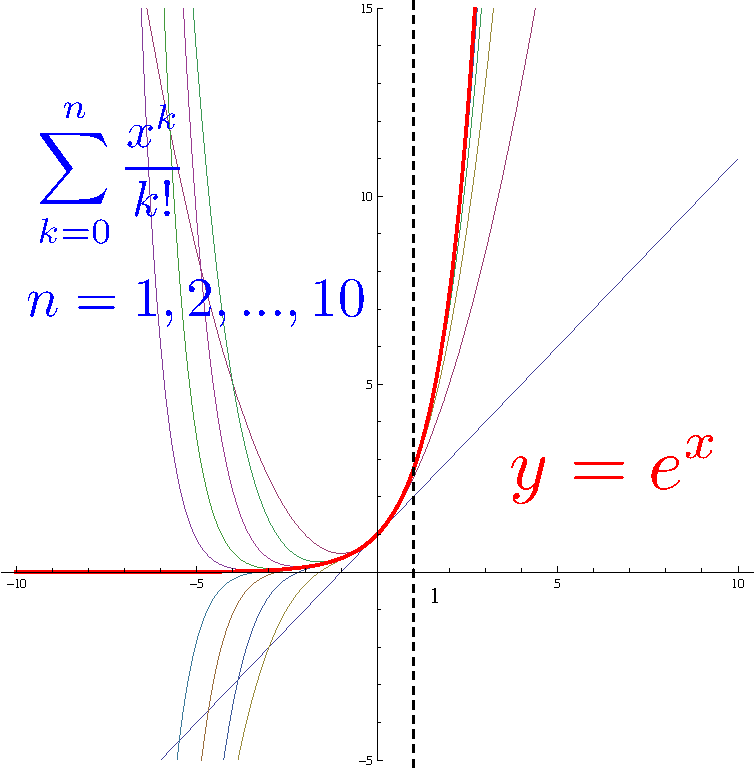
\includegraphics{./images/ch5/exse1.pdf}}\quad
	\resizebox{!}{5.5cm}{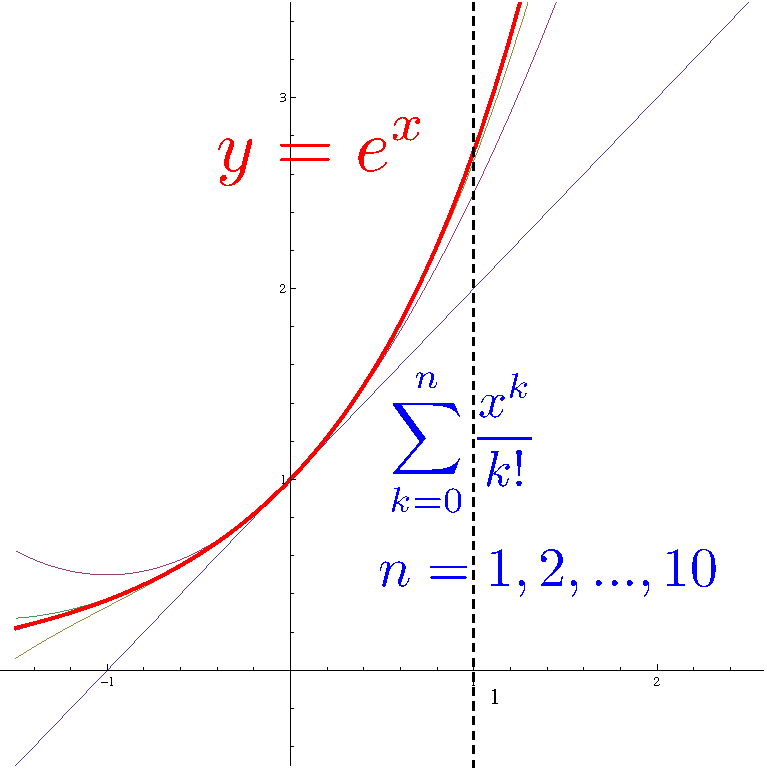
\includegraphics{./images/ch5/exse2.pdf}}
\end{center}

\subsubsection{计算不定式极限}

要证明Taylor公式的强大,用它来计算各种不定式极限无疑是最好的途径。某种意义上说,
没有用Taylor公式无法解决的极限问题,关键的问题是,值不值得动用这个“{\it 牛刀杀鸡}”。

{\bf 例:}计算以下极限
\begin{enumerate}[(1)]
  \setlength{\itemindent}{1cm}
  \item $\limx{0}\df{x-\sin x}{x^3}
  =\limx0\df{x-[x-\frac{x^3}3!+\circ(x^3)]}{x^3}=\df16$
  \item $\limx{0}\df{\cos x-e^{-x^2/2}}{x^4}
  =\limx0\df{1-\frac{x^2}2+\frac{x^4}{4!}-[1-\frac{x^2}2+
  \frac{x^4}8]+\circ(x^4)}{x^4}=-\df1{12}$ 
  \item $\limx{0}\df{\df{x^2}{2}+1-\sqrt{1+x^2}}{x^2\sin x^2}
  =\limx0\df{\frac{x^2}2+1-[1+\frac12{x^2}-\frac18x^4+\circ(x^4)]}{x^4}
  =\df18$ 
  \item $\limx{0}\df{e^x-1-x}{\df{1}{\sqrt{1+x}}-\cos\sqrt x}
  =\limx0\df{\frac{x^2}2+\circ(x^2)}{1-\frac12x+\frac38x^2-[1-\frac{x}2+\frac{x^2}{4!}]+\circ(x^2)}
  =\df32$ 
  \item $\limx{0}\df{\cos(\sin x)-\cos x}{x^4}
  =-2\limx0\df{\sin\frac{\sin x+x}2\sin\frac{\sin x-x}2}{x^4}=\df16$
  \item $\limx{+\infty}\left[x-x^2\ln\left(1+\df 1x\right)\right]
  \xlongequal{u=1/x}\lim\limits_{u\to0}\df{u-\ln(1+u)}{u^2}$
\end{enumerate}

从解题的过程来看,对于各种“$\df{\bm0}{\bm0}$”型的不定式极限,都可以先将分子分母
都展开成Taylor公式,然后通过简单的有理函数极限运算求得结果。因此,在此类极限问题上,
我们说Taylor是“{\it 万能}”的也并不为过。

然而,Taylor公式“{\it 天生}”比我们此前接触的计算工具更复杂
(这完全是因为它推广或者说蕴含了过去的大部分结论),因此在使用它时也需要加倍地谨慎。
在对分子分母进行Taylor展开时,一般都需要作一些“试探性”地尝试,
确定上下各展开到多少阶合适(太低解决不了问题,太高计算过于复杂),当然,
最重要的是,必须确保每一个展开式都精确无误。

最后,提醒一点,在Taylor展开中,灵活地进行高阶无穷小的合并,也是非常重要的。

{\bf 例:}设$f(x)$在$x=0$附近二次可导,且
$$\limx{0}\left(1+x+\df{f(x)}{x}\right)^{1/x}=e^3,$$
求:
\begin{enumerate}[(1)]
  \setlength{\itemindent}{1cm}
  \item $f(0),f\,'(0),f\,''(0)$;
  \item $\limx{0}\left(1+\df{f(x)}{x}\right)^{1/x}$.
\end{enumerate}

[解]:注意到$1/x\to\infty\;(x\to0)$,故已知极限存在,当且仅当
$$\limx0\left(1+x+\df{f(x)}x\right)=1
\quad\Rightarrow\quad f(0)=\limx0f(x)=0.$$
又原式即为
$$\left\{\limx0\left(1+x+\df{f(x)}{x}\right)
^{\frac{x}{x^2+f(x)}}\right\}^{\limx0\frac{x^2+f(x)}{x^2}}=e^3,$$
故必有
$$\limx0\frac{x^2+f(x)}{x^2}=3\quad\Rightarrow\quad
\limx0\df{f(x)}{x^2}=2,$$
进而
$$f'(0)=\limx0\df{f(x)-f(0)}x=\limx0\df{f(x)}{x^2}\limx0x=0.$$
至此,由Taylor公式,可设$f(x)=\df{f''(0)}2x^2+\circ(x^2)$,于是
$$2=\limx0\df{f(x)}{x^2}=\df{f''(0)}2\quad\Rightarrow\quad
f''(0)=4.$$
综上,$f(x)=2x^2+\circ(x^2)$,
\begin{align}
	\limx{0}\left(1+\df{f(x)}{x}\right)^{1/x}
	&=\limx0(1+2x+\circ(x))^{\frac1x}\notag\\
	&=\left\{\limx0(1+2x+\circ(x))^{\frac1{2x+\circ(x)}}\right\}
	^{\limx0{[2+\circ(1)]}}=e^2.\notag	
\end{align}
\hfill$\Box$

{\bf 例:}设$x\to 0$时,$e^{\tan x}-e^x$与$x^n$为同阶无穷小,则$n$=(C)
\ps{Taylor展开}

\quad
(A)\;$1$\hspace{2cm}
(B)\;$2$\hspace{2cm}
(C)\;$3$\hspace{2cm}
(D)\;$4$ 

% {\bf 例:}设$x\to 0$时,$x-\sin ax$与$x^2\ln(1-bx)$为同阶无穷小,则(A)
% \ps{Taylor展开}
% 
% \quad
% (A)\;$a=1,b=-\df16$\hspace{1em}
% (B)\;$a=1,b=\df16$\hspace{1em}
% (C)\;$a=-1,b=-\df16$\hspace{1em}
% (D)\;$a=-1,b=\df16$

\subsubsection{证明等式或不等式}

{\bf 例:}证明:$x>0$时,$e^x>1+x+\df{x^2}{2}$

[证]:$x>0$时,由Taylor公式,存在$\xi\in(0,x)$,使得
$$e^x=1+x+\df{x^2}2+\df{e^{\xi}}{3!}x^3>1+x+\df{x^2}2.$$
即证。\hfill$\Box$

{\bf 例:}设$f(x)$在$(a,+\infty)$内具有二阶导数,
且$f(x),f\,''(x)$在$(a,+\infty)$
有界,证明:$f\,'(x)$在$(a,+\infty)$有界。

[证]:由$f(x)$和$f''(x)$有界,可知存在$M>0$,对任意$x>a$,均有
$$|f(x)|\leq M,\quad |f''(x)|\leq M.$$
对任意$x>a$,有如下的Taylor公式:存在$\xi\in(x,x+1)$,使得
$$f(x+1)=f(x)+f'(x)+\df12f''(\xi).$$
从而可知
$$f'(x)=f(x+1)-f(x)-\df12f''(\xi),$$
进而有
\begin{align*}
	|f'(x)|&=|f(x+1)-f(x)-\df12f''(\xi)|
	\leq |f(x+1)|+|f(x)|+\df12|f''(\xi)|\\
	&\leq M+M+\df12M=\df52M.
\end{align*}
这意味着$f'(x)$当$x>a$时有界,即证。\hfill$\Box$

从上面的例题不难看出,{\b 用Taylor公式证明等式和不等式,因为涉及到具体的估计和放缩,
都必须使用Lagrange余项}。

{\bf 例:}证明:若在$(a,b)$内,$f''(x)>0$,则对任意$a<x_1<x_2<b$,恒有
$$f\left(\df{x_1+x_2}{2}\right)<\df{f(x_1)+f(x_2)}{2}.$$

[证]:记$c=\df{x_1+x_2}2$,则由Taylor公式,存在$\xi_1\in(x_1,c),
\xi_2\in(c,x_2)$,使得
$$f(x_1)=f(c)+f'(c)\df{x_1-x_2}2+f''(\xi_1)
\left(\df{x_1-x_2}2\right)^2$$
$$f(x_2)=f(c)+f'(c)\df{x_2-x_1}2+f''(\xi_2)
\left(\df{x_2-x_1}2\right)^2$$
两式相加,且由$f''(x)>0$,可得
$$f(x_1)+f(x_2)=2f(c)+[f''(\xi_1)+f''(\xi_2)]
\left(\df{x_2-x_1}2\right)^2>2f(c),$$
即证。\hfill$\Box$

{\bf 思考:}本例的结论可以进一步推广为:对任意$\lambda\in(0,1)$,
$$f(\lambda x_1+(1-\lambda)x_2)<\lambda
f(x_1)+(1-\lambda)f(x_2).$$
请考虑该如何证明。

% {\bf 例:}设在$f(x)$在$[0,a]$上二阶连续可导,
% $|f\,''(x)|\leq M$,且$|f(x)|$在$(0,a)$内可取到最大值,证明:
% $$|f\,'(0)+f\,'(a)|\leq Ma.$$
% 
% [提示]:将$f'(0)$和$f'(a)$在最大值点处展开,然后将两个展开式合并即可。

{\bf 例:}设$f(x)$在$[0,1]$上二阶连续可导,且$f(0)=f(1)$,
$|f\,''(x)|\leq A$,证明:对任意$x\in(0,1)$,恒有
$$|f\,'(x)|\leq\df A4.$$

[证]:由Taylor公式,对任意$x\in(0,1)$,存在$\xi_1\in(0,x),
\xi_2\in(x,1)$,使得
$$f(0)=f(x)+f'(x)(-x)+\df{f''(\xi_1)}2x^2,$$
$$f(1)=f(x)+f'(x)(1-x)+\df{f''(\xi_2)}2(1-x)^2,$$
两式相减,且由$f(0)=f(1)$,可得
$$0=f'(x)+\df12\left[f''(\xi_2)(1-x)^2-f''(\xi_1)x^2\right],$$
由$|f''(x)|\leq A$,故
$$|f'(x)|\leq\df A2[(1-x)^2+x^2],$$
注意到当$x\in(0,1)$时,$(1-x)^2+x^2\leq1$,故$|f'(x)|\leq\df A2$,即证。
\hfill$\Box$

通过上面的例题,可以总结一下使用Taylor公式证明等式和不等式的一些规律:
{\b
\begin{itemize}
  \item 如果同时涉及到多个不同阶的导数,可以考虑使用Taylor公式;
  \item 必须使用带Lagrange余项的Taylor公式;
  \item 展开和被展开点的常见选择: 区间端点、 极(最)值点、
  区间中点、 距离为常数的点、 已知条件中提到的特殊点。
\end{itemize}
}

{\bf 例:}设$f(x)\in C^3[-1,1]$,且$f(-1)=0,f(1)=1,f'(0)=0$,
证明:存在$\xi\in(-1,1)$,使得$f'''(\xi)=3$.

[提示]:将$f(-1),f(1)$在$x=0$处展开到三阶带Lagrange余项的Taylor公式,
然后利用介值定理。

{\bf 例:}\ps{辅导书P153-例37}
设$f(x)$在$[a,b]$上二阶连续可导,且$f_+'(a)=f_-'(b)=0$,则至少存在一点
$c\in(a,b)$,使得
$$|f\,''(c)|\geq \df 4{(b-a)^2}|f(b)-f(a)|.$$

[提示]:将$f\left(\df{a+b}2\right)$在$x=a,b$展开,取绝对值放缩后,
利用介值定理。

\begin{ext}
	{\bf 课后作业}
	
	\begin{enumerate}
	  \item 求$f(x)=x^4+x^3-2x-4$在$x=0$和$x=2$处的三阶Taylor多项式。
	  \item 求函数$f(x)=\df1{x-1}$按$(x-2)$的幂展开的带有Peano余项的
	  $n$阶Taylor公式。
	  \item 求如下函数带Peano余项的Maclaurin公式
		\begin{enumerate}[(1)]
% 		  \setlength{\itemindent}{1cm}
		  \item $\ln(2+x^2)$
		  \item $e^{\frac{x^2}2}$
		  \item $x\cos x^2$
		  \item $\df{1+x^2}{1-x^2}$
		  \item $\df1{\sqrt{4-x^2}}$
		  \item $\sin^2x-x^3$
		  \item $(1+x)e^{x}$
		\end{enumerate}
	  \item 计算如下极限
	  \begin{enumerate}[(1)]
% 		\setlength{\itemindent}{1cm}
		\item $\limx{+\infty}(\sqrt[3]{x^3+3x^2}-\sqrt[4]{x^4-2x^3})$
		\item $\limx0\df{\cos x-e^{-\frac{x^2}2}}{x^2[x+\ln(1-x)]}$
		\item $\limx0\df{1+\frac12x^2-\sqrt{1+x^2}}{(\cos x-e^{x^2})\sin x^2}$
		\item $\limx{+\infty}\left[\left(x^3-x^2+\df{x}2\right)e^{\frac1x}
		-\sqrt{x^6+1}\right]$
	  \end{enumerate}
	  \item 应用$3$阶Taylor公式计算$\sqrt[3]{30}$的近似值,并估计其误差。
	  \item 设$x\to 0$时,$x-\sin ax$与$x^2\ln(1-bx)$为同阶无穷小,求$a,b$的值。
	  \item 已知$f(x)$在$x=0$附近二阶可导,且
	  $$\limx0\left[\df{\sin x}{x^3}+\df{f(x)}{x^2}\right]=0,$$
	  求$\limx0\left[\df3{x^2}+\df{f(x)}{x^2}\right]$。
	  \item (选作)证明:若在$(a,b)$内,$f''(x)>0$,则对任意$a<x_1<x_2<b$,恒有:
	  对任意$\lambda\in(0,1)$,
		$$f(\lambda x_1+(1-\lambda)x_2)<\lambda
		f(x_1)+(1-\lambda)f(x_2).$$
	  \item (选作) 设在$f(x)$在$[0,a]$上二阶连续可导,
		$|f\,''(x)|\leq M$,且$|f(x)|$在$(0,a)$内可取到最大值,证明:
		$$|f\,'(0)+f\,'(a)|\leq Ma.$$		
		[提示]:将$f'(0)$和$f'(a)$在最大值点处展开,然后将两个展开式合并即可。
	\end{enumerate}
\end{ext}

\section{函数的单调性与凹凸性}

\subsection{单调性的判定}

利用Lagrange中值定理,可以很容易地证明如下结论:若$f(x)$在$[a,b]$上连续,
$(a,b)$内可导,且$f\,'(x)$恒大(小)于零,则$f(x)$在$[a,b]$上严格单调递增(减)。

需要注意的是,这仅仅是判定可导函数严格单调的充分条件,而非充要条件
(例如:$f(x)=x+\sin x$严格单调递增,但导数可能为零)。
当然,如果定理中的“大(小)于”改成“大(小)于等于”,
且结论改为(非严格的)单调递增(减)情形,则为充要条件。

仔细观察可以发现,如果定理中的“大(小)于”改成“大(小)于等于”,且导数不可能在任何一段
连续区间内恒等于零,则可推出函数为{\it 严格}单调的。

\begin{thx}
	{\bf 可导函数严格单调的充要条件:}设$f(x)$在$[a,b]$上连续,$(a,b)$内可导,
	则$f(x)$在$[a,b]$上严格单调递增,当且仅当:
	\begin{enumerate}[(1)]
% 	  \setlength{\itemindent}{1cm}
	  \item $f\,'(x)\geq 0,\;x\in(a,b)$
	  \item 在$(a,b)$的任意子区间上$f\,'(x)$不恒为零
	\end{enumerate}
\end{thx}

利用该结论,可以很方便地证明类似如下的例子:

{\bf 例:}讨论$y=x-\sin x$的单调性。

\begin{center}
	\resizebox{!}{5cm}{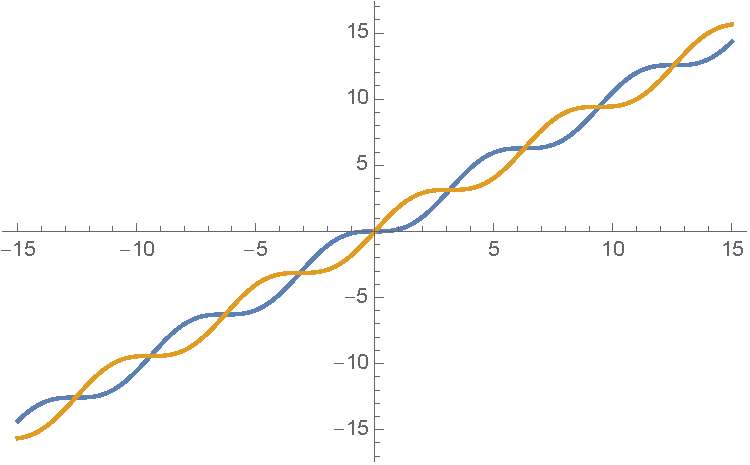
\includegraphics{./images/ch5/xpmSinx.pdf}}
	
	{\it $y=x\pm\sin x$的函数图形}
\end{center}

\subsubsection{单调性的应用}

证明不等式是单调性最常见的一种应用:

\begin{thx}
	{\bf 推论1:}设$\varphi(x),\psi(x) $均在$[a,b]$上可导,且:
	\begin{enumerate}[(1)]
% 	  \setlength{\itemindent}{1cm}
	  \item $\varphi'(x)>\psi'(x),\;x\in(a,b)$;
	  \item $\varphi(a)\geq\psi(a)$,
	\end{enumerate}
	则在$(a,b)$上,恒有$\varphi(x)>\psi(x)$。
\end{thx}

{\bf 例:}证明:当$x>0$时,恒有
$$x-\df 16x^3<\sin x<x.$$

\begin{center}
	\resizebox{!}{5cm}{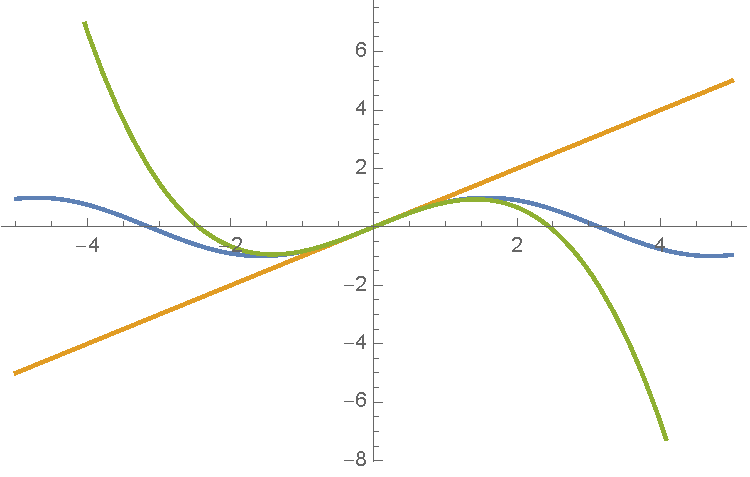
\includegraphics{./images/ch5/xSinxx3.pdf}}
\end{center}

很多时候,为了证明不等式,需要多次应用以上的结论,从而有如下的推论:

\begin{thx}
	{\bf 推论2:}设$\varphi(x),\psi(x) $均在$[a,b]$上$n$阶可导,且:
	\begin{enumerate}[(1)]
% 	  \setlength{\itemindent}{1cm}
	  \item $\varphi^{(n)}(x)>\psi^{(n)}(x),\;x\in(a,b)$;
	  \item $\varphi^{(k)}(a)\geq\psi^{(k)}(a),k=0,1,2,\ldots,n-1$,
	\end{enumerate}
	则在$(a,b)$上,恒有$\varphi(x)>\psi(x)$。
\end{thx}


{\bf 例:}证明下列不等式
\begin{enumerate}[(1)]
  \setlength{\itemindent}{1cm}
  \item $\ln(1+x)>\df{\arctan x}{1+x},\;(x>0)$
  \item $e^x>1+x+\df
  {x^2}{2!}+\df{x^3}{3!}+\ldots+\df{x^n}{n!},\;(x>0,n\in\mathbb{N})$
\end{enumerate}

\begin{center}
	\resizebox{!}{4cm}{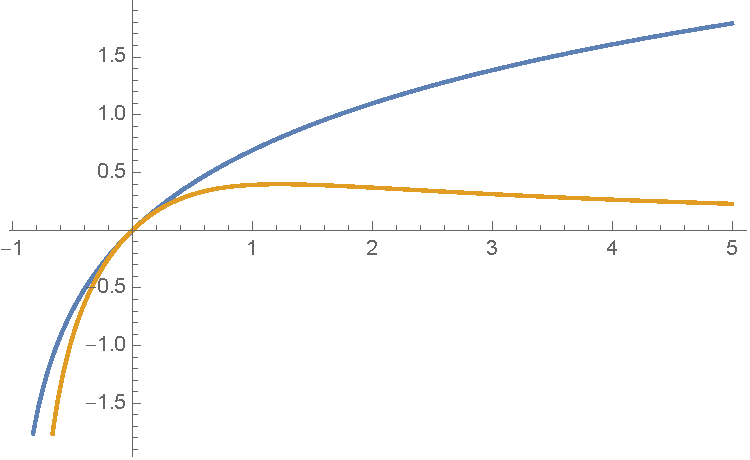
\includegraphics{./images/ch5/lnxArctanx.pdf}}\quad
	\resizebox{!}{4cm}{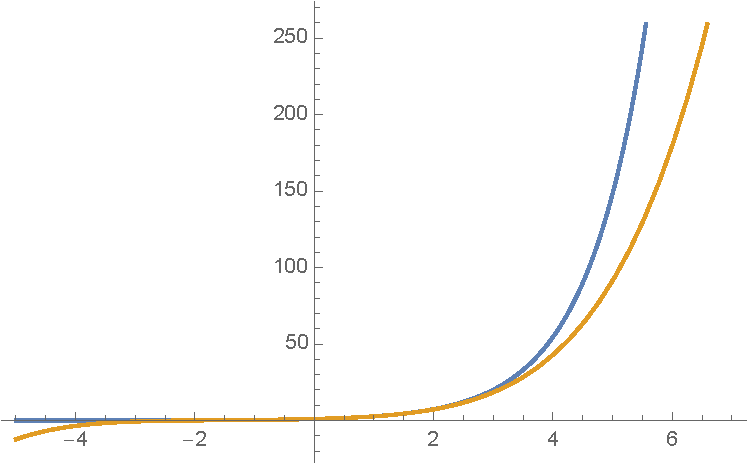
\includegraphics{./images/ch5/exTaylor.pdf}}
\end{center}

此外,单调性也常常用来判定解的唯一性,例如:

{\bf 例:}已知$x>0$时,
$$kx+\df1{x^2}=1$$
有且仅有一个根,求$k$的取值范围。\ps{此类题目的叙述一定要注意逻辑表达,
既要避免过于繁琐,也要防止遗漏重要的论证}

解:令$f(x)=kx^3-x^2+1\;(x>0)$。显然原方程在$x>0$内有且仅有一个根,
当且仅当$f(x)$在$x>0$内有唯一零点。

(1)$k\leq 0$时,$f(+\infty)=-\infty$,注意到$f(0+0)=1$,
故由介值定理,$f(x)$在$x>0$上至少有一个零点。又当$x>0$时,
$f'(x)=(3kx-2)x<0$,故$f(x)$严格单调递减,从而以上零点唯一;

(2)$k>0$时,$f(+\infty)=+\infty$,令$f'(x)=0$,可得$x=\df2{3k}$
为$f(x)$的在$x>0$内的唯一驻点,又$f''\left(\df2{3k}\right)=2>0$,
故$x=\df2{3k}$为$f(x)$的最小值点。$f_{\min}=f\left(\df2{3k}\right)=1
-\df4{27k^2}$,由此可知:

若$k<\df29\sqrt3$,则$f_{\min}<0$,由介值定理,$f(x)$至少有两个零点;

若$k>\df29\sqrt3$,则$f_{\min}>0$,则当$x>0$时$f(x)>0$,无零点;

若$k=\df29\sqrt3$,则$x=\df2{3k}$为$f(x)$的唯一零点。

综上,当$k\leq 0$或$k=\df29\sqrt3$即为所求。\hfill$\Box$

\subsection{凹凸性与拐点}

任给一条平面曲线,从几何的角度我们可能会这样看待它,它是平直的还是弯曲的?
它向什么方向弯曲和倾斜?它的平滑程度如何?它有多长?

通过前面的学习,我们已经了解了,导数可以用来刻画曲线的倾斜程度(斜率),
同时告诉我们曲线本身是否平滑。但是,这还只是部分地回答了上面的问题。
本小结我们将关注的焦点集中在曲线弯曲的问题上,从凹凸的角度来刻画曲线
的几何特征。对于剩余的问题,我们将会再本章稍后的内容中继续加以讨论。

% {\bf 约定:}以下的凹凸均指“上凹”和“上凸”\ps{\b 目前的教材上对于函数的凹凸和
% 曲线的凹凸定义有所不同,并且刚好相反:K}

对于凹凸这样的几何特征,通过观察我们可以这样加以描述,以凹为例:一段曲线称为
是凹的,可以理解为{\it 连接其上任意两点的曲线段总是位于连接两点的线段的下方}(可以重叠)。

\begin{center}
 	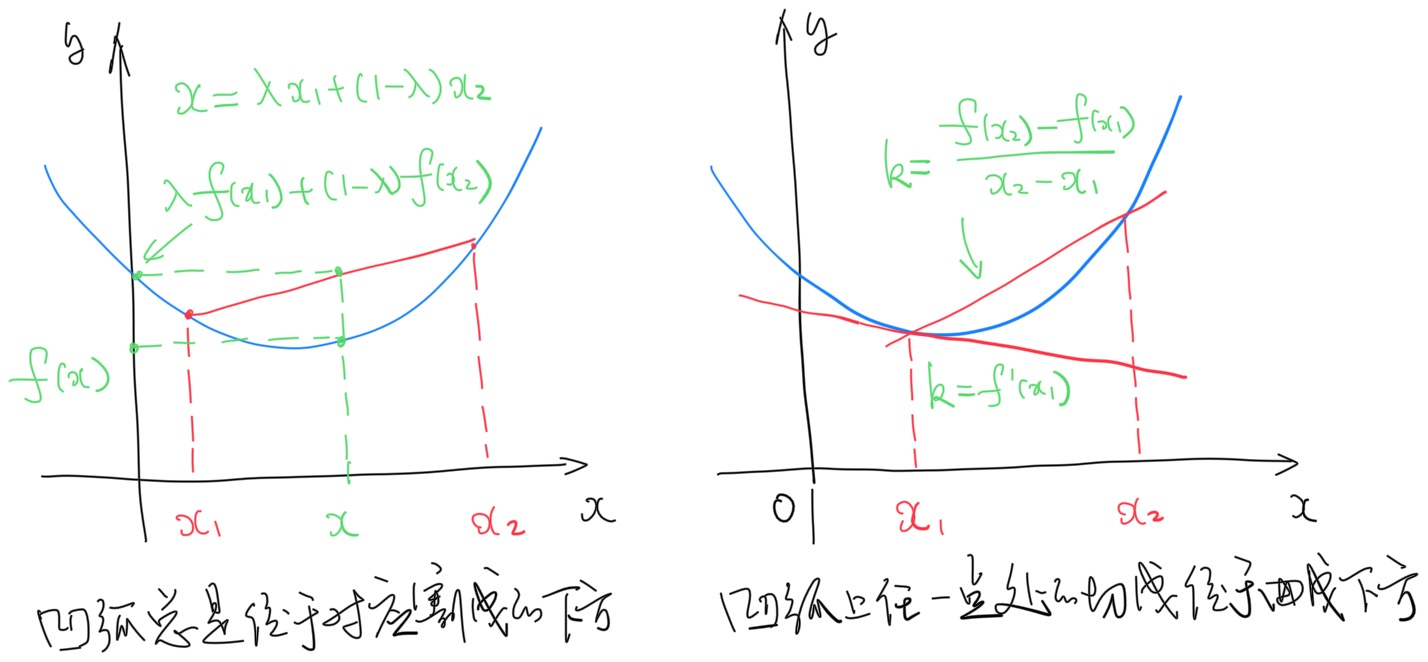
\includegraphics[width=0.9\textwidth]{./images/ch3/convexCurve.jpg}

	\kaishu 凹弧的几何特征
\end{center}

对于这一性质在数学上可以表达为:

\begin{thx}
	设函数$f(x)$在区间$I$上有定义,若对任意$x_1,x_2\in I$,
	以及任意$\lambda\in(0,1)$,有
% 	\ps{\b 直观地说,就是割线上的取值大于函数值,则称为凹,反之为凸}
	$$f[\lambda x_1+(1-\lambda)x_2]\leq\lambda f(x_1)+(1-\lambda)f(x_2)$$
	则称$f(x)$的图形在区间$I$上的是{\bf 凹弧}。若上式中的等号严格成立,则称其为
	{\bf 严格的凹弧}。类似地,可以定义{\bf 凸弧}和{\bf 严格的凸弧}。
\end{thx}
{\bf 注:}同济教材中的定义相当于取定$\lambda=\df12$,考虑到$x_1,x_2$的任意性,
其定义和以上的定义是完全等价的。请思考一下如何证明这一点?

显然,从定义上看,一段曲线是否为凹(凸)弧,与其是否是光滑的无关。事实上,由多段
折线连接而成的一段曲线也可能是凹(凸)的,但不可能是严格凹(凸)的(想想为什么?)。
而如果一段曲线具有较好的光滑性(可导性),能够对我们判定其凹(凸)提供更大的便利。

\begin{thx}
	{\bf 凹弧判定的充要条件:}
	设$f(x)$在$(a,b)$内可导,则$f(x)$的曲线在$(a,b)$是凹弧,当且仅当:
	对任意$x_1,x_2\in(a,b)$,恒有
	$$f(x_2)\geq f(x_1)+f\,'(x_1)(x_2-x_1). $$
	不等号严格成立时,对应于严格凹函数的情形。
\end{thx}
这个定理的含义是:{\it 凹弧上任意点处的切线总是位于曲线的下方}。

[证]:若$f(x)$的曲线为凹的,则对任意$x_1,x_2\in(a,b)$和任意$t\in[x_1,x_2]$,有
$$f(t)\leq\df{x_2-t}{x_2-x_1}f(x_1)+\df{t-x_1}{x_2-x_1}f(x_2)
=f(x_1)+\df{f(x_2)-f(x_1)}{x_2-x_1}(t-x_1),$$
从而
$$\df{f(t)-f(x_1)}{t-x_1}\leq\df{f(x_2)-f(x_1)}{x_2-x_1},$$
由极限的保号性,令$t\to x_1^+$,可得
$$f'(x_1)\leq\df{f(x_2)-f(x_1)}{x_2-x_1},$$
也即
$$f(x_2)\geq f(x_1)+f\,'(x_1)(x_2-x_1).$$

另一方面,由Lagrange中值定理,对任意$x_1,x_2\in(a,b)$,存在
$\xi\in(a,b)$,使得
$$\df{f(x_2)-f(x_1)}{x_2-x_1}=f'(\xi),$$
也即
$$f(x_2)=f(x_1)+f'(\xi)(x_2-x_1).$$

于是由
$$f(x_2)\geq f(x_1)+f\,'(x_1)(x_2-x_1)$$
可得
$$f'(x_1)\leq\df{f(x_2)-f(x_1)}{x_2-x_1}=f'(\xi).$$
从而
$$f(x_2)\geq f(x_1)+f'(x_1)(x_2-x_1).$$
\hfill$\Box$

这个定理虽然给出了凹弧判定的充要条件,但从结论的形式上看,是非常不易验证的。
如果进一步知道$f(x)$是二阶可导的,可以使用如下更为简单的判定方法:

\begin{thx}
	{\bf 凹凸性判定的充分条件:}
	设$f(x)$在$(a,b)$二阶可导,则
	\begin{enumerate}[(1)]
% 	  \setlength{\itemindent}{1cm}
	  \item 若$f\,''(x)$恒不小于零,$f(x)$为凹函数;
	  \item 若$f\,''(x)$恒不大于零,$f(x)$为凸函数。
	\end{enumerate}
\end{thx}

这个定理的证明需要用到Taylor公式,在第3.3节我们已经以例题的形式证明过,在此
不再重复。

一段曲线常常是由多段凹弧和凸弧相接构成的,例如:$y=x^3$的曲线在$x<0$的部分
是凸的,在$x>0$的部分是凹的。位于凹、凸弧交界处的点,我们一般称之为曲线的{\bf 拐点},
如果曲线在改点是二阶可导的,容易推出在该点处二阶导数为零。例如$x=0$就是$y=x^3$
对应曲线的拐点。但特别需要注意的是,二阶导数为零的点,不一定都是曲线的拐点。例如
$y=x^4$在$x=0$处二阶导数为零,但该点并不是对应曲线的拐点,而是一个{\it 极小值点}。

事实上,{\it\b 要判定一个点是否为曲线的拐点,只需判断一下在该点左右的二阶导数是否符号是相异的}。

\begin{shaded}
	{\bf 讨论:}由$f''(x_0)=0$是否可以推出$x=x_0$为拐点?

	[答]:不能!例如$y=x^3$和$y=x^4$,在$x=0$处,前者为拐点,后者是极值点!
	具体可参照如下的分析方法:
	\begin{center}
	\begin{tabular}{c||c|c|c|c}
		\hline 
		$f(x)=x^3$ & $x<0$ & $x=0$ & $x>0$ & \\ 
		\hline 
		$f(x)$ & - & 0 & + & \\ 
		\hline 
		$f'(x)$ & + & 0 & + & 拐点\\ 
		\hline 
		$f''(x)$ & - & 0 & + & \\ 
		\hline 
		$f'''(x)$ & + & + & + & \\ 
		\hline 
		 &  &  &  &  \\ 
		\hline 
	\end{tabular} 
	\begin{tabular}{c||c|c|c|c}
		\hline 
		$f(x)=x^4$ & $x<0$ & $x=0$ & $x>0$ & \\ 
		\hline 
		$f(x)$ & + & 0 & + & 极小值\\ 
		\hline 
		$f'(x)$ & - & 0 & + & \\ 
		\hline 
		$f''(x)$ & + & 0 & + & \\ 
		\hline 
		$f'''(x)$ & - & 0 & + & \\ 
		\hline 
		$f^{(4)}(x)$ & + & + & + & \\ 
		\hline 
	\end{tabular} 
	\end{center}
	
	综合来看,$f''(x)=0$的点只能作为可能的拐点,并且,拐点也可能出现在不可导点处。
\end{shaded}

{\bf 例:}证明一个三次多项式对应的曲线只有唯一的拐点,如果它有三个根$x_1,x_2,x_3$,
则拐点的横坐标一定是$\df13(x_1+x_2+x_3)$。

\begin{ext}
	{\bf 课后作业}
	
	\begin{enumerate}
	  \item 证明下列不等式
		\begin{enumerate}[(1)]
% 		  \setlength{\itemindent}{1cm}
		  \item 当$x\in(0,\pi/2)$时,$\sin x+\tan x>2x$
		  \item 当$x>0$时,$1+x\ln(x+\sqrt{1+x^2})>\sqrt{1+x^2}$
		\end{enumerate}
	  \item 求下列函数图形的拐点
	  \begin{enumerate}[(1)]
% 		\setlength{\itemindent}{1cm}
		\item $y=(x+1)^4-e^x$
		\item $y=e^{\arctan x}$
		\item $y=xe^{-x}$
	  \end{enumerate}
	  \item 设$x,y>0$,证明如下不等式
	  \begin{enumerate}[(1)]
		\item $x^{100}+y^{100}\geq\df{(x+y)^{100}}{2^{99}}$
		\item $x\ln x+y\ln y\geq (x+y)\ln\df{x+y}2$
	  \end{enumerate}
	  \item 设$f(x)$当$x\geq a$时二阶可导,且$f''(x)>0$,证明:
	  $F(x)=\df{f(x)-f(a)}{x-a}$当$x>a$时单调递增。
	\end{enumerate}
\end{ext}

\section{函数的极值与最值}

在现实中,最值问题无处不在,应用广泛。从数学的角度,很多时候可以抽象为所谓
的极值和最值问题。

{\bf 例:}画出函数$f(x)=3x^4-4x^3-12x^2+3$在区间$[-2,3]$上的图形,通过
观察求其最大和最小值。

如图
\begin{center}
	\resizebox{!}{5cm}{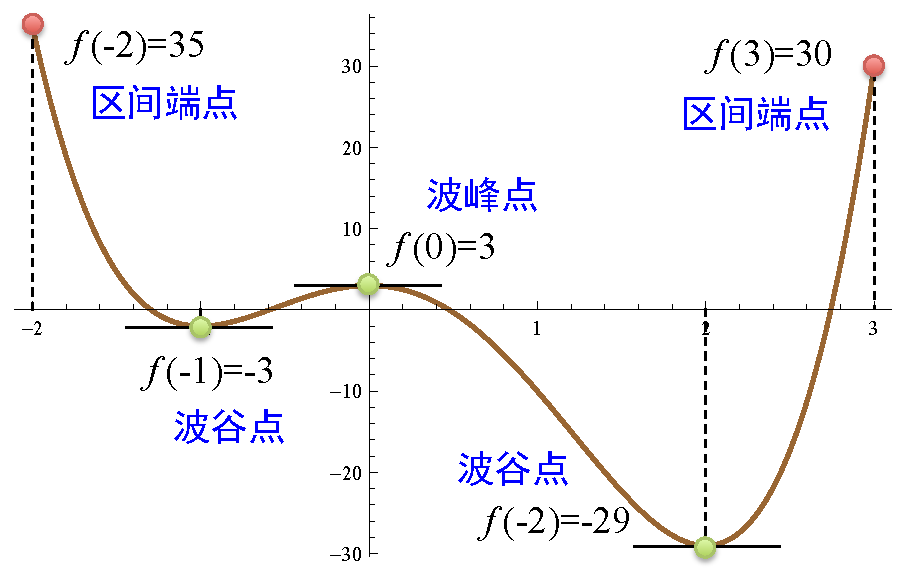
\includegraphics{./images/ch5/fmm_pt.pdf}}
	
	$f(-2)=35,\quad f(3)=30,\quad f(2)=-29$
\end{center}

从图上不难看出一些“潜在”的极值和最值点,通过对这些点处的函数值加以比较,
能容易得出函数的最大和最小值。而图上标出的“波峰”和“波谷”,则对应于我们
所说的极值点。

\subsection{极值}

我们这里所说的极值,也即{\it 局部唯一的最值},其定义如下:

\begin{thx}
	设在$x_0$的某去心邻域内,恒有
	$$f(x)<f(x_0)\quad (\mbox{或}\quad f(x)>f(x_0)),$$
	则称$f(x_0)$是$f(x)$的一个{\bf 极大(小)值},$x_0$称为
	$f(x)$的一个{\bf 极值点}。
\end{thx}

显然,
\begin{itemize}
  \setlength{\itemindent}{1cm}
  \item 函数在极值点处未必可导; 
  \item 可导函数极值点处的导数为零——{\kaishu Fermat引理};
  \ps{Fermat引理也称为{\bf 极值判定的必要条件}} 
  \item 导数为零的点(称为{\bf 驻点})未必是极值点。
\end{itemize}

关于最后一条,结合几何图形进行观察,
\begin{center}
	\resizebox{!}{4cm}{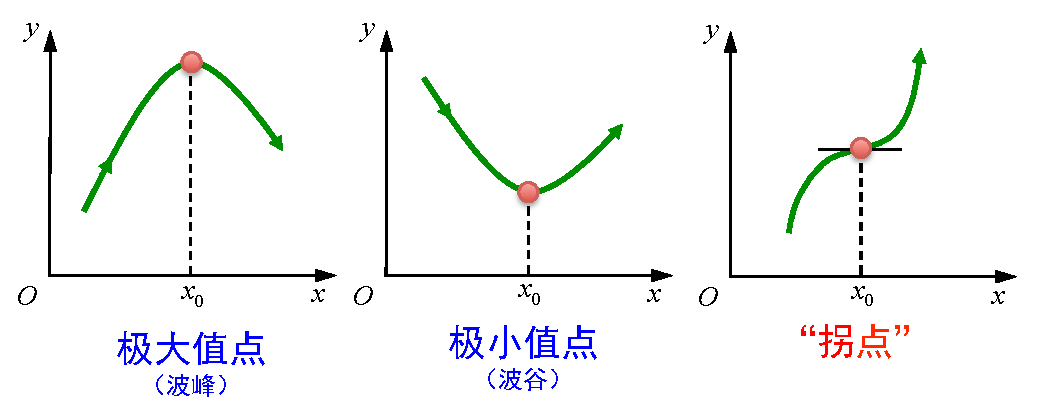
\includegraphics{./images/ch5/edge_pt.pdf}}
\end{center}
不难发现,驻点可能是极值点,也可能不是(这时称为{\bf 拐点})。

\begin{thx}
	{\bf 连续函数极值的充分条件:}设$f(x)$在$x_0$附近连续,
	若$f(x)$在$x_0$两侧单调性相反,则$f(x)$在$x_0$取极值。
\end{thx}

{\bf 思考:}以上定理表明,{\it 连续函数单调性的分界点是函数的极值点。}
那么,这个条件是充要的吗?

[答]:函数的极值点可能在不连续的点上取到,这时不必要求在极值点两侧的单调性不同。
例如:$f(x)=x-[x]$,在每个整数点上都取极小值,但在极值点两侧都是严格单调递增的。

\begin{thx}
	{\bf 可导函数极值的第一充分条件:}设$f(x)$在$x_0$附近可导,
	且$f'(x)$在$x_0$两侧符号相反,则$f(x)$在$x_0$处取极值。
\end{thx}

结合几何图形,不难看出,如果$f'(x)$在$x_0$左侧为正,右侧为负,则$x_0$
为$f(x)$的极大值点;反之为极小值点。

{\bf 例:}讨论以下函数的极值
\begin{enumerate}[(1)]
  \setlength{\itemindent}{1cm}
  \item $f(x)=2-|x^3-1|$
  \item $f(x)=\left(1+x+\df{x^2}{2!}+\ldots+\df{x^n}{n!}\right)e^{-x}$ 
\end{enumerate}

\begin{center}
	\resizebox{!}{4cm}{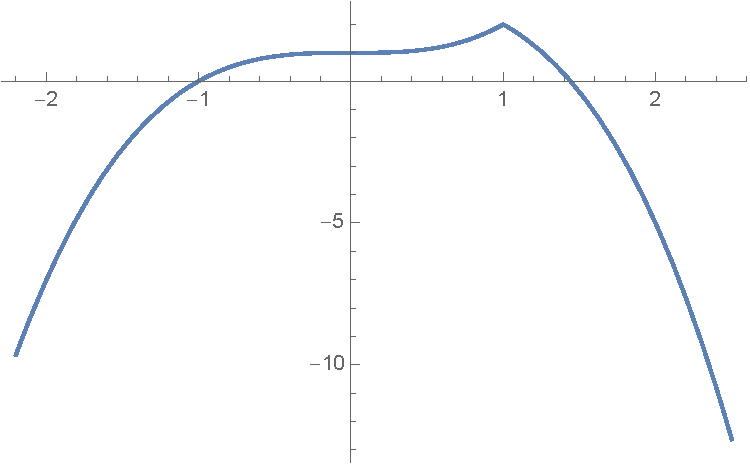
\includegraphics{./images/ch5/2x3.pdf}}\quad
	\resizebox{!}{4cm}{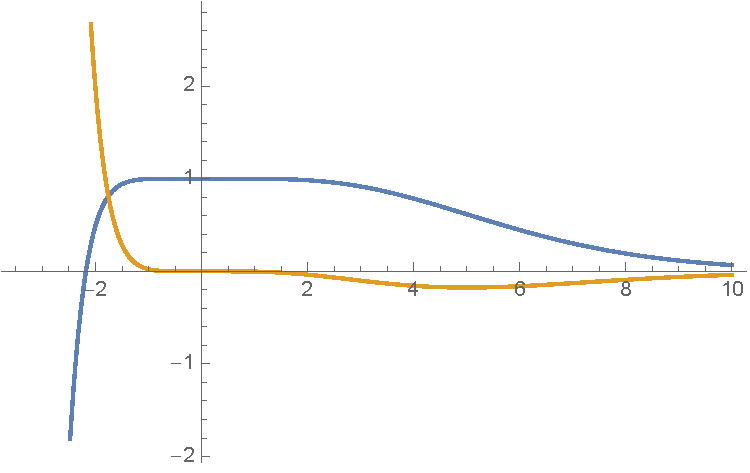
\includegraphics{./images/ch5/1xxe-x.pdf}}
	
	{\it 蓝色和黄色分别为函数和导函数的曲线}
\end{center}

\begin{thx}
	{\bf 可导函数极值的第二充分条件:}设$f(x)$在$x_0$处二阶可导,
	且$f'(x_0)=0$,$f''(x_0)\ne 0$,则
	\begin{enumerate}[(1)]
	  \item 若$f''(x_0)<0$,则$x_0$为$f(x)$的极大值点;
	  \item 若$f''(x_0)>0$,则$x_0$为$f(x)$的极小值点;
	\end{enumerate}
\end{thx}

注意,{\b 对于$f'(x_0)=f''(x_0)=0$的情况,定理中没有涉及,其结论并不是
$x_0$不是$f(x)$的极值点,而应该说此时无法判定$x_0$是不是$f(x)$的极值点!}

例如考虑$f_1(x)=x^3$和$f_2(x)=x^4$,在$x=0$处,两个函数的一二阶导数
都为零,但是从图像上很容易看出,$x=0$是后者的极小值点,而不是前者的极值点。
要给出这样的判断,方法其实并不复杂,通常使用可导函数极值的第一充分条件即可,
如果仍然无法判定,再考虑其他特殊的方法。

\begin{shaded}
	{\it(参见: 明万元,黄香蕉,一种判断多项式函数极值点和拐点个数的简单方法,
	大学数学,2011年,第27卷第6期,161-163)
	
	http://www.doc88.com/p-0651660157725.html}
	$$P(x)=\prod_{i=1}^n(x-a_i)^{p_i}$$
	其中$a_i\in\mathbb{R}$,$p_i\in\mathbb{Z}^+\;(i=1,2,\ldots,n)$
	且$a_1<a_2<\ldots<a_n$。
	
	记$a_{i_1},\ldots,a_{i_k}$为$P(x)$的重根,$l$为其中三重根的个数。
	
	{\bf 命题:}{\bf 多项式函数的拐点、极值点判定}
	\begin{enumerate}
  	  \setlength{\itemindent}{1cm}
	  \item $P(x)$有且仅有$k+(n-1)$个驻点,包括:
	  \begin{itemize}
	    \setlength{\itemindent}{0.5cm}
	    \item $k$个重根:$a_{i_1},\ldots,a_{i_k}$
	    \item 介于两个零点之间的:$\xi_i\in(a_i,a_{i+1}),\;i=1,2,\ldots,n-1$
	  \end{itemize}
	  \item 以上所有的驻点中
	  \begin{itemize}
	    \setlength{\itemindent}{0.5cm}
	    \item 若$p_{i_j}(j=1,2,\ldots,k)$为偶数,则$a_{i_j}$为$P(x)$的极值点
	    \item 若$p_{i_j}(j=1,2,\ldots,k)$为奇数,则$a_{i_j}$为$P(x)$的拐点
	    \item $\xi_i\in(a_i,a_{i+1}),\;i=1,2,\ldots,n-1$均为极值点
	  \end{itemize}
	  \item $P''(x)$有且仅有$l+(k+n-2)$个零点
	  \begin{itemize}
	    \setlength{\itemindent}{0.5cm}
	    \item $l$个三重根
	    \item 介于每两个相邻驻点之间的:$\eta_i,\;i=1,2,\ldots,k+n-2$
	  \end{itemize}
	\end{enumerate}
	
	综上,对于前述的多项式函数,可以得出这样一些常用的{\it 判定准则}:
	\begin{tcolorbox}
		{\bf 多项式函数极值与拐点的判定:}
		\begin{enumerate}[(1)]
% 	  	  \setlength{\itemindent}{1cm}
		  \item 所有二次以上的重根均为驻点,其中偶数次的为极值点,奇数次的为拐点;
		  \item 两个相邻零点之间有且仅有一个极值点;
		  \item 两个相邻驻点之间有且仅有一个拐点。
		\end{enumerate}
	\end{tcolorbox}	
	
	{\bf 例:}$y=(x-1)(x-2)^2(x-3)^3$有几个极值点和拐点?
	
	\begin{center}
		\resizebox{!}{5cm}{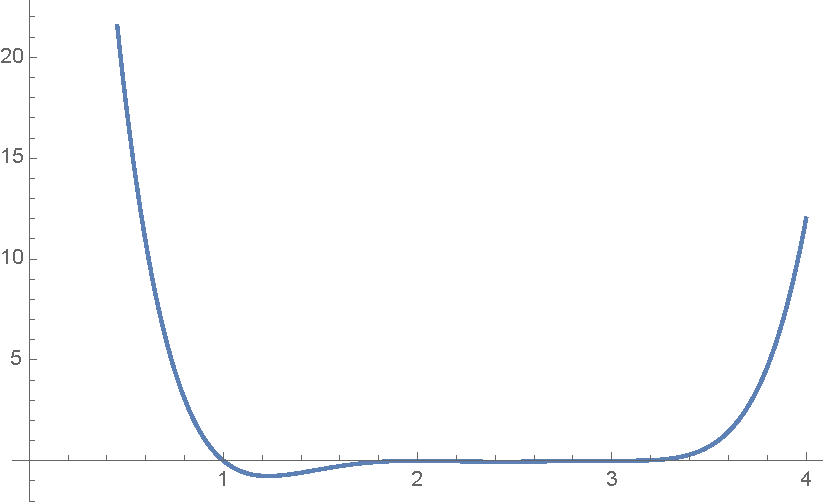
\includegraphics{./images/ch5/x123.pdf}}
	\end{center}
	
	{\bf 解:}利用前述的判定准则:
	\begin{enumerate}[(1)]
  	  \setlength{\itemindent}{1cm}
	  \item $x=2$为$2$重根,故为驻点兼极值点
	  \item $x=3$为$3$重根,故为驻点兼拐点
	  \item 在$(1,2)$和$(2,3)$中各有一个驻点兼极值点,记为$\xi_1,\xi_2$
	  \item $4$个驻点由小到大的排列为
	  $$\xi_1<2<\xi_2<3,$$
	  故在其间有且仅有$3$个拐点
	\end{enumerate}
	
	综上,该函数共有$3$个极值点,$4$个拐点。
	
	{\bf 例:}$y=2(x+1)^5(x-2)^8(x-4)^3+9$有几个极值点和拐点?
	
	\begin{center}
		\resizebox{!}{5cm}{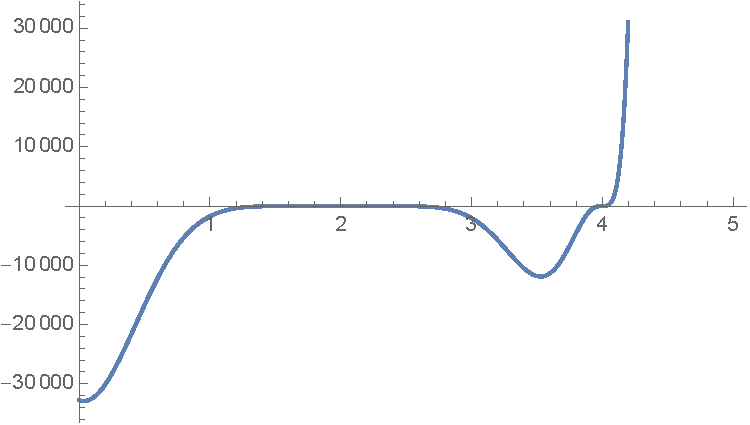
\includegraphics{./images/ch5/x124.pdf}}
	\end{center}
	
	{\bf 解:}注意到该函数和
	$$y=2(x+1)^5(x-2)^8(x-4)^3,$$
	的极值点和拐点完全相同,故我们只需研究后者的极值点和拐点个数:
	\begin{enumerate}[(1)]
  	  \setlength{\itemindent}{1cm}
	  \item $x=-1$为$5$重根,故为驻点兼拐点
	  \item $x=2$为$8$重根,故为驻点兼极值点
	  \item $x=4$为$3$重根,故为驻点兼拐点
	  \item 在$(-1,2)$和$(2,4)$中各有一个驻点兼极值点,记为$\xi_1,\xi_2$
	  \item $5$个驻点由小到大的排列为
	  $$-1<\xi_1<2<\xi_2<4,$$
	  故在其间有且仅有$4$个拐点
	\end{enumerate}
	
	综上,该函数共有$3$个极值点,$6$个拐点。
	
\end{shaded}

{\bf 例:}讨论以下函数的极值
\begin{enumerate}[(1)]
  \setlength{\itemindent}{1cm}
  \item $f(x)=x^3-6x^2+5$\hfill (教材-例4)
  \item $f(x)=\cos x+\df12\cos 2x$
\end{enumerate}

\begin{center}
	\resizebox{!}{4cm}{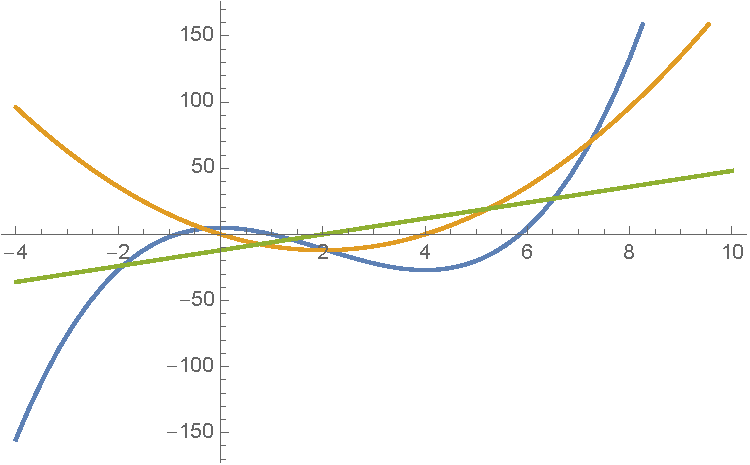
\includegraphics{./images/ch5/x36x2-5.pdf}}\quad
	\resizebox{!}{4cm}{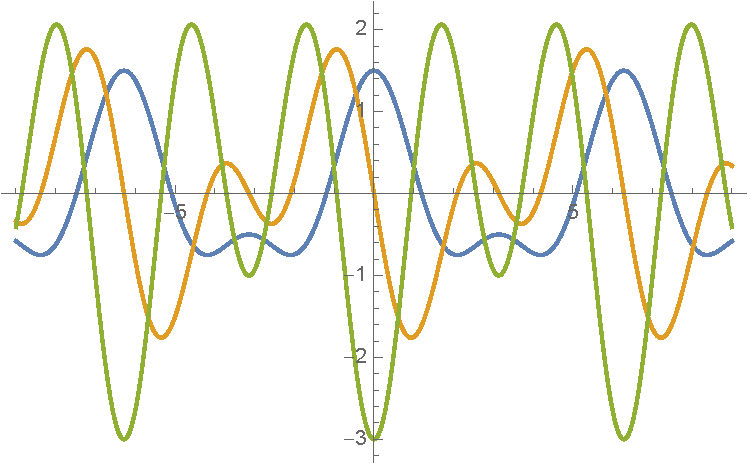
\includegraphics{./images/ch5/cosxcos2x.pdf}}
	
	{\it 蓝色、黄色和绿色分别为函数、导函数和二阶导函数的曲线}
\end{center}

\begin{thx}
	{\bf 求给定函数极值的一般步骤}
	\begin{enumerate}[(1)]
	  \item 在$f(x)$的可导区间上,求解$f'(x)=0$,找出其所有的驻点;
	  \item 利用可导函数极值的第二充分条件,找出驻点中的极值点;
	  \item 对于$f(x)$的所有不可导点,以及上一步中无法判定的点($f''(x)=0$),
	  如果$f(x)$在这些点附近连续或可导,则利用连续函数极值的
	  充分条件或可导函数极值的第一充分条件,判定其是否为极值;
	  \item 如果仍存在无法判定的情况,可考虑使用极值的定义,或引入其他特殊
	  的方法进行判定。	  
	\end{enumerate}
\end{thx}

{\bf 例:}求函数$f(x)=(x^2-1)^3$的极值。

{\bf 例:}判断正误
\begin{enumerate}[(1)]
  \setlength{\itemindent}{1cm}
  \item {\b 函数的极大值一定是最大值\quad  ({$\times$})} 
  \item {\b 函数的最大值一定是极大值\quad  ({$\times$})} 
  \item {\b 函数的极大值一定比极小值大\quad  ({$\times$})} 
\end{enumerate}

{\bf 例:}函数$f(x)$对满足
$$xf\,''(x)+3x[f\,'(x)]^2=1-e^{-x}$$
\begin{enumerate}[(1)]
  \setlength{\itemindent}{1cm}
  \item 若$f(x)$在$x=c\ne 0$处有极值,证明其必为极小值;
  \item 若$f(x)$在$x=0$处有极值,该极值为极大还是极小?
\end{enumerate}

{\bf 例:}求数列$\sqrt[n]n$中最大的一项。

\begin{center}
	\resizebox{!}{5cm}{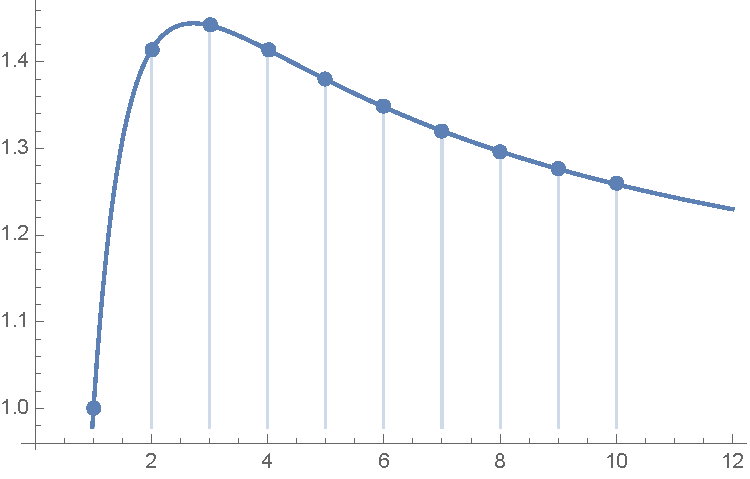
\includegraphics{./images/ch5/x1x.pdf}}
\end{center}

{\bf 例:}求$a$的取值范围,使$y=a^x$与$y=x$必相交。

[提示]:充要条件是存在$x_0>0$,满足$a^{x_0}=x_0$,也即$a$位于$g(x)=x^{x}$
的值域中。结果$a\in(0,e^{\frac1e}]$

{\bf 例:}判定方程$2^x-2x=1$有几个实根。

\begin{center}
	\resizebox{!}{5cm}{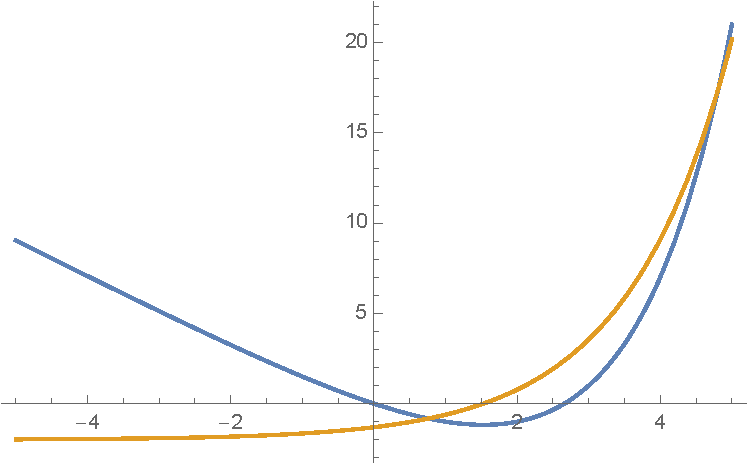
\includegraphics{./images/ch5/2x2x.pdf}}
\end{center}

{\bf 例:}设$a,b$均为正数,证明:$a(1-b)$和$b(1-a)$不可能同时大于$\df14$。

[提示]:令$f(x)=x(1-x)$,可求得其最大值为$\df14$。若以上两数都大于$1/4$,则
$$a(1-b)b(1-a)>\df1{16},$$
这与前述最大值的性质矛盾。

{\bf 注:}更直观的解法是,假设结论不成立,则
$$a>\df14+ab,b>\df14+ab\quad\Rightarrow\quad
ab>\left(\df14+ab\right)^2,$$
进而可得
$$\left(\df14-ab\right)^2<0,$$
出现错误,故假设不成立。

% {\bf 例:}当$a$取何值时,$a^x\geq1+x$恒成立。
% 
% [提示]:两条曲线总有交点$(0,1)$,又$(a^x)''=a^x\ln^2x>0$,故$y=a^x$上凹。
% 要使之位于$y=x+1$上方,只需后者为其切线,由此易得$a=e$.

\begin{shaded}
{\bf 证明平均值不等式}

{\bf 例:}证明:$\df{x_1+x_2+\ldots+x_n}n\geq\sqrt[n]{x_1x_2\ldots x_n}$,
其中$x_1,x_2,\ldots,x_n$均为正数。

[证]:$n=2$时,设$f(x)=\df{x_1+x}2-\sqrt{x_1x}$,则
$$f'(x)=\df12\left(1-\sqrt{x_1}x\right),$$
$x=x_1$为唯一驻点,又$f''(x_1)>0$,故$f(x_1)$为最小值点。

设$n=k$时,命题成立。令
$$f(x)=\df{x_1+x_2+\ldots+x_k+x}{k+1}-\sqrt[k+1]{x_1x_2\ldots x_kx},$$
于是
$$f'(x)=\df1{k+1}\left[1-\df{{x_1x_2\ldots x_k}^{\frac1{k+1}}}
{x^{\frac k{k+1}}}\right],$$
$x_0=\sqrt[k]{x_1x_2\ldots x_k}$为唯一驻点,且$f''(x_0)>0$,故$f(x_0)$为最小值。
$$f(x_0)=\df1{k+1}(x_1+x_2+\ldots+x_k-k\sqrt[k]{x_1x_2\ldots x_k})\geq 0$$
即证。
\end{shaded}

% {\bf 例:}$a$取何值时,$f(x)=2x^3-9x^2+12-a$恰有两个零点(B)
% 
% A)$2$\quad B)$4$\quad C)$6$\quad D)$8$

[提示]:$f'(x)=6(x-2)(x-1)$,$x=1,2$为极值点,若$f(1)$或$f(2)$为零,即有结论成立。

{\bf 例:}$f(x)=|x(1-x)|$,则$x=0$(C)
\begin{enumerate}[A)]
  \setlength{\itemindent}{1cm}
  \item 是极值点,但不是拐点
  \item 不是极值点,但是拐点
  \item 是极值点,也是拐点
  \item 不是极值点,也不是拐点
\end{enumerate}

% {\bf 例:}$f(x)$二阶导数连续,$f'(0)=0$,$\limx{0}\df{f''(x)}{|x|}=1$,
% 则(B)
% \begin{enumerate}[A)]
%   \setlength{\itemindent}{1cm}
%   \item $f(0)$是$f(x)$的极大值点
%   \item $f(0)$是$f(x)$的极小值点
%   \item $f(0)$是$f(x)$的拐点
%   \item $f(0)$不是极值点,也不是拐点
% \end{enumerate}

\subsection{最值(最优化)问题}

显然,所有极值点都可以视为“候选”的最值点。幸运的是,由于最大和最小值的判定
是非常直观的(直接比较函数值的大小),最值的问题通常显得比极值问题更为简单。

给定一个区间$I$,要求给定函数$f(x)$在其上的最值,首先需要找出所有可能的
最值点。

\begin{center}
	\resizebox{!}{4cm}{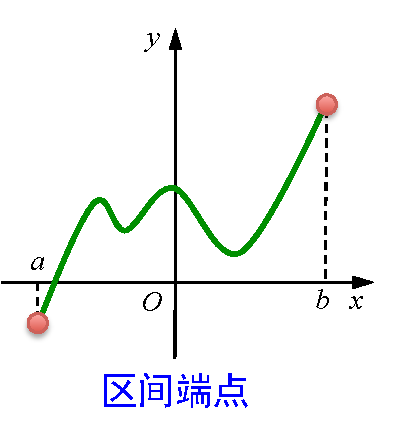
\includegraphics{./images/ch5/mm1.pdf}}
	\resizebox{!}{4cm}{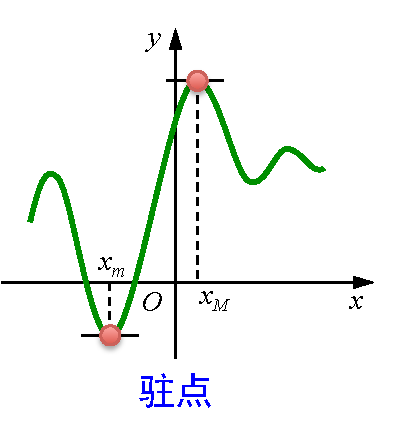
\includegraphics{./images/ch5/mm2.pdf}}
	\resizebox{!}{4cm}{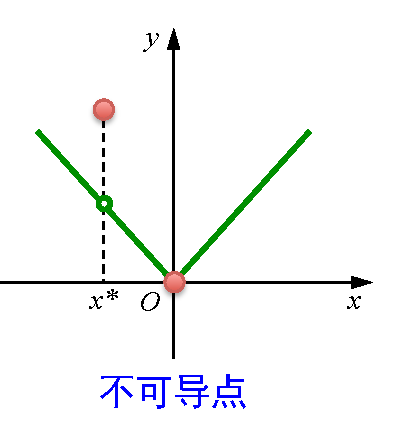
\includegraphics{./images/ch5/mm3.pdf}}
\end{center}

\begin{thx}
	{\bf 求连续函数$f(x)$在闭区间$[a,b]$上的最值:}
	\begin{enumerate}[(1)]
% 	  \setlength{\itemindent}{1cm}
	  \item 确定函数在区间内的所有{\it 驻点}和{\it 不可导点}:
	  $x_1,x_2,$ $\ldots,x_n$ 
	  \item 逐个计算
	  $f(a),f(x_1),f(x_2),\ldots,f(x_n),f(b)$,
	  比较以上函数值,确定最大和最小值。
	%   \ps{之所以不考虑其他的点,是因为这些点没有考虑的价值}
	\end{enumerate}
\end{thx}

{\bf例:}求函数$f(x)=3x^4-4x^3-12x^2+3$在区间$[-2,3]$上的最大和最小值。

\begin{shaded}
	{\bf 优化问题:}
	
	最值问题的另一个名称是优化问题,通常是指,在给定条件下
	求特定函数的最值(最优解)的问题。形式上,可以这样来描述:
	
	\begin{tcolorbox}
		{\bf 目标:}求函数$f(x_1,x_2,\ldots,x_n)$的最值;
	
		{\bf 约束:}变量$x_1,x_2,\ldots,x_n$所需满足的条件,
		例如:取值范围或者需要满足的方程(不等式)
	\end{tcolorbox}
	现实中的优化问题多不胜数,例如:	
	\begin{itemize}
% 	  \setlength{\itemindent}{1cm}
	  \item 给定边长,求所能围成的矩形区域的最大面积?
	  \item 给定一块正方形薄片,所能制成的无盖容器的最大容积?
	  \item 求给定圆中面积最大的正多边形,或者反之,求给定多边形中最大的内接圆?
	  \item 给定一定的原材料,组合生产各种商品所能获得最大利润?
	  \item 为了达到特定生产收益,最少需要投入多少资源?
	  \item 给定燃料总量,规划最优路线,使得行驶距离最远?
	  \item \ldots \ldots
	\end{itemize}
	
	本章我们所讨论的是优化问题中最简单的一类,即{\it 单变量单目标的优化问题},
	在现实的优化问题中,常常涉及大量的变量,变量之间可能存在错综复杂的约束关系,
	优化的目标也不是单一的变量(所谓的{\it 多目标优化})。	更多地时候,
	优化问题本身是作为一门学科或一个研究领域,而不是一个单一的问题而存在的。
\end{shaded}

\begin{thx}
	{\bf 求解最值(优化)问题的一般步骤:}
	\begin{enumerate}[(1)]
% 	  \setlength{\itemindent}{1cm}
	  \item 理解题意:画图、定义变量;
	  \item 建立关系:给出目标函数和约束条件的表达式;
	  \item 求解最值:推理(或仿真)求解。
	\end{enumerate}
\end{thx}


{\bf 例:}一个边长为$a$的方形铁皮,在四角各剪去一个边长为$x$的小正方形,然后折成
一个无盖的长方体容器,问当$x$取何值时,长方体容器的容积最大?

{\bf 例:}半径为$R$的圆形纸张上剪去一个扇形,剩余部分做成一个圆锥形容器,求该容器的最大
容量。

[提示]:设余下的圆心角为$2\pi-\theta$,于是圆锥的底边长伟$\theta R$,从而
底面半径为$r=\df{\theta}{2\pi}R$,圆锥的高$h$满足
$$h^2=R^2-r^2=R^2\left(1-\df{\theta^2}{4\pi^2}\right),$$
圆锥体积的平方为
$$V^2(\theta)=\df{\pi^2R^6}9\left(\df{\theta^2}{4\pi^2}\right)^2
\left(1-\df{\theta^2}{4\pi^2}\right)$$
记$x=\df{\theta^2}{4\pi^2},c=\df{\pi^2R^6}9$,从而$V=cx^2(1-x)$,显然$x\in[0,1]$,
计算可得其驻点$x_0=\df23$,易证其也是最大值点,此时$V_{\max}=\df{2\pi R^3}{9\sqrt3}$

[例]:用输油管连接离海岸12km的钻井平台和沿岸往下20km处的炼油厂。已知水下和陆上铺设
管道的成本分别是每公里50万元和30万元,问该如何设计线路,使总的建设成本最低?

{\bf 例(地质勘探):}通常情况下,声波上层岩石中的传播速度$c_1$小于在下层岩石中的传播速度$c_2$。
如图所示,求
\begin{enumerate}[(1)]
  \setlength{\itemindent}{1cm}
  \item 用$d,h,c_1,c_2$和$\theta$表示$T_1,T_2,T_3$
  \item 证明$\sin\theta=\df{c_1}{c_2}$时,$T_2$最小
  \item 假设$d=1km,T_1=0.26s,T_2=0.32s,T_3=0.34s$,求$c_1,c_2,h$
\end{enumerate}
\begin{center}
	\resizebox{!}{4cm}{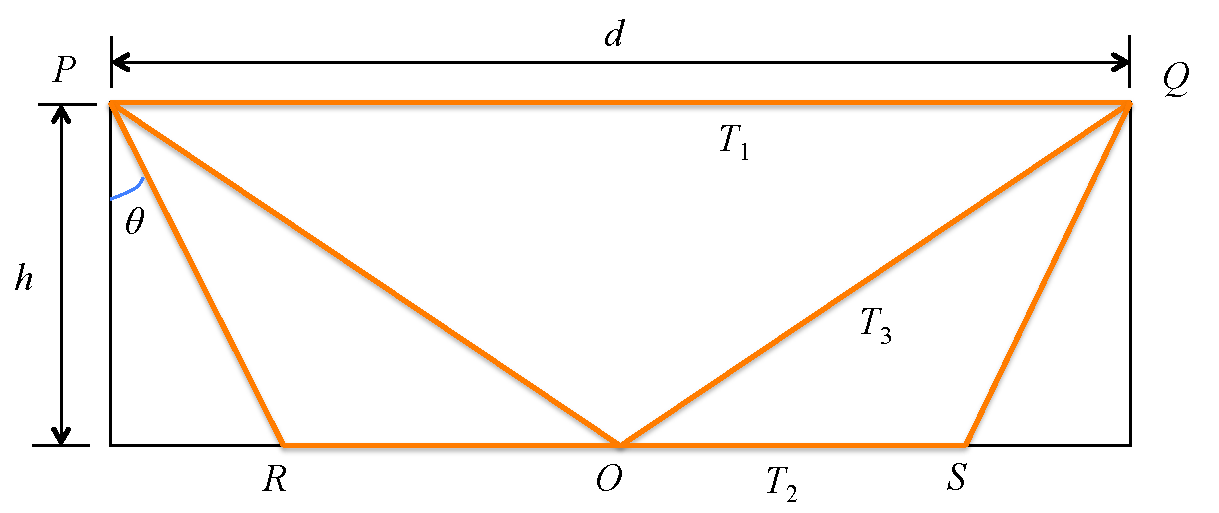
\includegraphics{./images/ch5/eWave.pdf}}
\end{center}

[提示]:(1)
$$T_1=\df d{c_1}$$
$$T_2=\df{2h}{c_1}\sec\theta-\df{2h}{c_2}\tan\theta+\df d{c_2}$$
$$T_3=\df2{c_1}\sqrt{h^2+\left(\df d2\right)^2}$$


(2)
$$\df{\d T_2}{\d\theta}=\df{2h(c_2\sin\theta-c_1)}{c_1c_2\cos^2\theta}$$
唯一驻点$\sin\theta=\df{c_1}{c_2}$,此时
$$T_2=\df{2h}{c_1c_2}\sqrt{c_2^2-c_1^2}+\df d{c_2}$$

(3)
$$c_1=\df{d}{T_1}\approx3.846km/s$$
$$h=\sqrt{\left(\df{c_1}2T_3\right)^2-\left(\df d2\right)^2}\approx0.4213km$$
又
$$(T_2c_2-d)^2=\df{4h^2}{c_1^2}(c_2^2-c_1^2)$$
解得$c_2=4.1024$或$7.6619$。

{\bf 例:}高度$h$的水桶,顶端不断注水使桶内总是保持水满的状态。在桶的侧面开个小孔,使水喷出。
若小孔距地面高度为$y$,则水喷出的速度为$8\sqrt{h-y}$。问小孔放在多高的位置,能使水喷出的距离
最远。

[提示]:$y\in(0,h)$,水落地的时间为$\sqrt{2y/g}$,从而喷出的距离
$$s(y)=\df{8\sqrt{2}}{\sqrt g}\sqrt{y(h-y)},$$
$s'(y)=\df{8\sqrt{2}}{\sqrt g}\df{h-2y}{2\sqrt{y(h-y)}}$,唯一驻点$y=\df h2$。
显然其为最大值点,$s_{\max}=\df{4\sqrt 2}{\sqrt{g}}h$

{\bf 例:}同一维度上两座建筑物,间隔$l=50$(m),高度分别为$h_1=60$(m)和
$h_2=30$(m),在两个建筑物间修一座太阳能
站,如何选址方为最优?

[提示]:使
$$\theta=\pi-\arctan\df{h_1}{x}-\arctan\df{h_2}{l-x}$$
最大。
$$\theta'_x=\df{h_1}{h_1^2+x^2}-\df{h_2}{h_2^2+(l-x)^2}$$
$$\left(x-\df{lh_1}{h_1-h_2}\right)^2-h_1h_2\left(\df{l^2}
{(h_1-h_2)^2}+1\right)=0$$

能保证最长的日照时间应为最优。结果为距较高的一侧约29.5m。

{\bf 例:}如图,从原点处发出的炮弹,求
\begin{enumerate}[(1)]
  \setlength{\itemindent}{1cm}
  \item 炮弹轨迹的参数方程
  \item 何时炮弹的射程最远
  \item 如果坡面是向上的呢?
\end{enumerate}
\begin{center}
	\resizebox{!}{5cm}{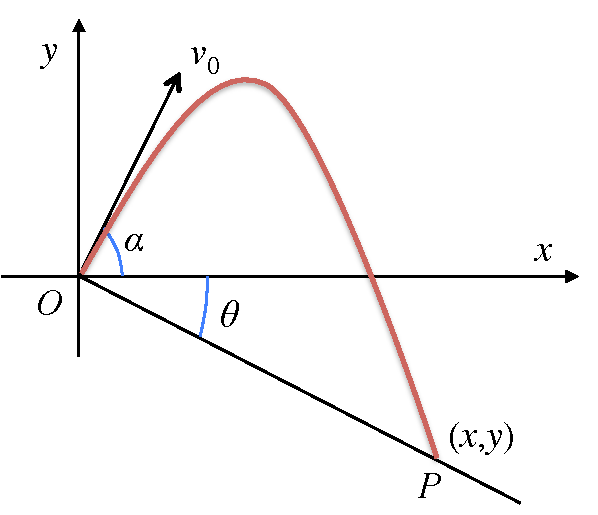
\includegraphics{./images/ch5/bFly.pdf}}
\end{center}

[提示]:(1)以时间$t$为参数,则
$$x=(v_0\cos\alpha)t,\quad y=(v_0\sin\alpha)t-\df12gt^2$$
消去$t$,可得$y=x\tan\alpha-\df{gx^2}{2v_0^2\cos^2\alpha}$。落点处满足
$y=-x\tan\theta$,联立解得
$$x=\df{2v_0^2\cos^2\alpha}g(\tan\alpha+\tan\theta),$$
从而炮弹的飞行时间
$$T=\df x{v_0\cos\alpha}=\df{2v_0\cos\alpha}g(\tan\alpha+\tan\theta),$$
从而参数$t\in[0,T]$。

(2)射程
$$R(\alpha)=x\sec\theta=\df{2v_0^2}{g\cos^2\theta}\cos\alpha\sin(\alpha+\theta),$$
$$R'(\alpha)=\df{2v_0^2}{g\cos^2\theta}\cos(2\alpha+\theta),$$
驻点$\alpha=\df12\left(\df{\pi}2-\theta\right)$

(3)使用$-\theta$替换$\theta$,最大值点$\alpha=\df12\left(\df{\pi}2+\theta\right)$

\begin{shaded}
{\bf 关于$\left(1+\df1n\right)^n\to e(n\to\infty)$的另一个证明}

{\bf 例:}$f_u(x)=x^ue^{-x}(x\geq0)$,对于确定的$u>0$,证明
\begin{enumerate}[(1)]
  \setlength{\itemindent}{1cm}
  \item $f_u(x)$在$x=u$处达到最大值;
  \item 由$f_u(u)>f_u(u+1)$和$f_{u+1}(u+1)>f_u(u)$推出
  $$\left(\df{u+1}u\right)^u<e<\left(\df{u+1}u\right)^{u+1}$$
  \item 由$\df{u}{u+1}<\left(\df{u+1}u\right)^u<e$推出
  $\lim\limits_{u\to+\infty}\left(1+\df1u\right)^u=e$
\end{enumerate}
\end{shaded}

% {\bf 例:}$a>1$,$x\in[0,1]$,证明:
% $$\df1{2^{a-1}}\leq x^a+(1-x)^a\leq 1$$
% 
% [提示]:令$f(x)=x^a+(1-x)^a$

% {\bf 例:}证明$x>0,y>0$时,$xy\leq x\ln x+e^{y-1}$
% 
% [提示]:证明$f(x)=\ln x+\df{e^{y-1}}x$最小值大于$y$即可。

{\bf 例:}$f_n(x)=\sin x+\sin^2x+\ldots+\sin^nx$,证明:
\begin{enumerate}[1)]
  \setlength{\itemindent}{1cm}
  \item $f_n(x)=1$在$\left(\df{\pi}6,\df{\pi}2\right)$内有且仅有一个根
  \item 设$x_n\in\left(\df{\pi}6,\df{\pi}3\right)$是以上的根,则$\limn x_n=\df{\pi}6$
\end{enumerate}

[提示]:1)介值定理,且$f(x)$严格单增;

2)$f_n\left(\df{\pi}{6}\right)=1-\df1{2^n}$,
$f'_n\left(\df{\pi}{6}\right)>\sqrt
3>1$,$n$充分大时 $$f'_n\left(\df{\pi}{6}+\df1{2^{n-1}}\right)
=f_n\left(\df{\pi}{6}\right)+f'_n\left(\df{\pi}{6}\right)\df1{2^{n-1}}
+\circ\left(\df1{2^{n-1}}\right)>1+\df1{2^n},$$
故$x_n\in\left(\df{\pi}{6},\df{\pi}{6}+\df1{2^{n-1}}\right)$

{\bf 例:}证明$x>0$时,$\df1{x(x+1)}>\ln^2(1+1/x)$

[提示]:令$y=1/x$,证明
$$y-\sqrt{1+y}\ln(1+y)>0$$

% {\bf 例:}证明:$\df{\tan x}x>\df x{\sin x}$,$x\in(0,\pi/2)$
% 
% 分析:$f(x)=\sin x\tan x-x^2$,$f(0)=f'(0)=f''(0)=0$,$f'''(x)>0$

{\bf 例:}$t\in[0,x]$,证明:$e^{-t}\geq\left(1-\df tx\right)^x$

[提示]:$t=0,x$时,显然成立。此外,设$f(x)=x\ln\left(1-\df tx\right)+t$,
则$\limx{+\infty}=0$,证明$f'(x)=\ln\left(1-\df tx\right)+\df t{x-t}>0$即可。

$u>0$时,$u>\ln(1+x)$,故
$$\df t{t-x}>\ln\left(1+\df t{x-t}\right)=-\ln\left(1-\df tx\right)$$

% {\bf 例:}比较$\pi^e$和$e^{\pi}$
% 
% 分析:令$f(x)=x-e\ln x$

\begin{ext}
	{\bf 课后作业}
	
	\begin{enumerate}
	  \item 求函数$f(x)=e^x+e^{-x}+\cos x$的极值。
	  \item 当$a$取何值时,$a^x\geq1+x$恒成立。
	  \item $a$取何值时,$f(x)=2x^3-9x^2+12-a$恰有两个零点。
	  \item 已知$f(x)$二阶导函数连续,$f'(0)=0$,$\limx{0}\df{f''(x)}{|x|}=1$,
	  证明$f(0)$是$f(x)$的极小值。
	  \item (选作)设$f(x)$在$x_0$处$n$阶可导,且
	  $$f'(x_0)=f''(x_0)=\ldots=f^{(n-1)}(x_0)=0,\;f^{(n)}(x_0)\ne 0,$$
	  证明:
	  \begin{enumerate}[(1)]
		\item 当$n$为奇数时,$f(x)$在$x_0$处不取极值;
		\item 当$n$为偶数时,$f(x)$在$x_0$处取极值,并且若$f^{(n)}>0$,
		$f(x_0)$为极小值,反之为极大值。
	  \end{enumerate}
% 	\end{enumerate}
% 	\tcblower
% 	\begin{enumerate}
	  \item 建造一个体积为$V$的圆柱体油罐,问该油罐的地面直径与高的比例为多少时,
	  所需要的建造材料最少。
	  \item 求曲线$x^2-xy+y^2=3$上横坐标最大和最小的点。
	  \item $a>1$,$x\in[0,1]$,证明:
	  $$\df1{2^{a-1}}\leq x^a+(1-x)^a\leq 1.$$
	  \item 比较$\pi^e$和$e^{\pi}$的大小。
	  \item 证明:$\df{\tan x}x>\df x{\sin x}$,$x\in(0,\pi/2)$。
	  \item (选作)证明$x>0,y>0$时,$xy\leq x\ln x+e^{y-1}$。
	\end{enumerate}
\end{ext}

\section{分析绘图}

{\bf 例:}已知多项式函数$f(x)$恰有两个极大值点和一个极小值点
\begin{enumerate}[(1)]
  \setlength{\itemindent}{1cm}
  \item 画出$f(x)$一个可能的图像
  \item 它最多有几个零点\hfill(4)
  \item 最少呢?\hfill(0)
  \item $f(x)$是奇数次还是偶数次的?\hfill(偶)
  \item 至少是多少次的?此时最多能有几个拐点?\hfill(4,4)
  \item 试给出一个它的表达式。\hfill($f(x)=(x-1)(x-2)(x-3)(x-4)$)
\end{enumerate}

% {\bf 例:}设函数$y=f(x)$具有如下性质,试作出其草图
% \begin{enumerate}[(1)]
%   \setlength{\itemindent}{1cm}
%   \item $f(x)$在$\mathbb{R}$上连续
%   \item $f(-4)=-3,f(0)=0,f(3)=2$
%   \item $f'(-4)=0,f'(3)=0$,且当$x\in(-\infty,-4)\cup(-4,-3)$时,$f'(x)>0$;
%   当$x\in(3,+\infty)$时,$f'(x)<0$
%   \item $f''(-4)=0,f''(0)=0$,切当$x\in(-\infty,-4)\cup(0,+\infty)$时,
%   $f''(x)<0$;$x\in(-4,0)$时,$f''(x)>0$
% \end{enumerate}

{\bf 例:}作出函数$y=\df{x}{1+x^2}$的图形。

\begin{center}
	\resizebox{!}{5cm}{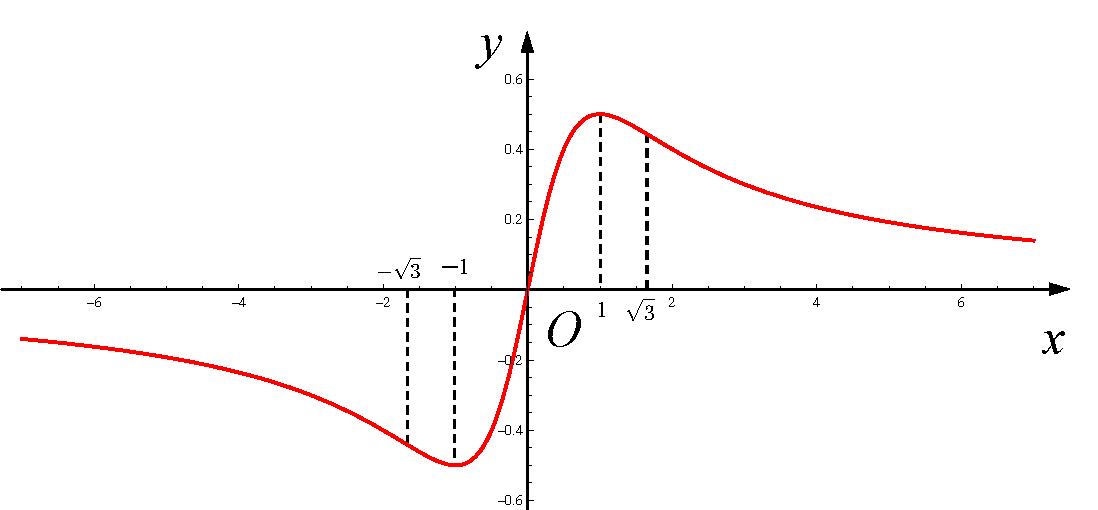
\includegraphics{./images/ch5/x1x2.pdf}}
\end{center}

\begin{thx}
	{\bf 分析绘图的一般步骤}
	\begin{enumerate}[(1)]
% 	  \setlength{\itemindent}{1cm}
	  \item {\bf 分析函数的简单性质:}定义域、值域、奇偶性、周期性、与坐标轴的交点;
	  \item {\bf 计算一、二阶导函数:}确定不可导点;
	  \item {\bf 列表分析:}标记出单调、凸凹区间,极值点和拐点;
	  \item {\bf 画出渐进线:}水平、铅直和斜渐进线;
	  \item {\bf 描点作图}。
	\end{enumerate}
\end{thx}

{\bf 例:}函数作图:$y=xe^{1/x}$
\begin{itemize}
  \setlength{\itemindent}{1cm}
  \item 极值点:$y(1)=e$
  \item 渐近线:$y=x+1$
\end{itemize}

\begin{center}
	\resizebox{!}{7cm}{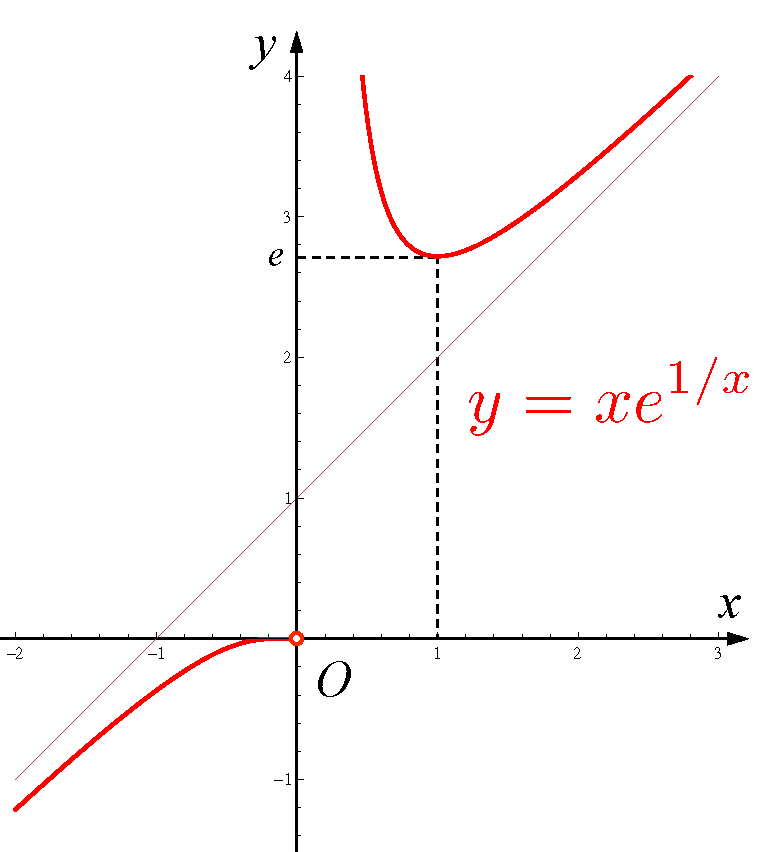
\includegraphics{./images/ch5/xe1x.pdf}}
\end{center}

\begin{ext}
	{\bf 课后作业}
	
	\begin{enumerate}
	  \item 设函数$y=f(x)$具有如下性质,试作出其草图
	  \begin{enumerate}[(1)]
% 		  \setlength{\itemindent}{1cm}
		  \item $f(x)$在$\mathbb{R}$上连续
		  \item $f(-4)=-3,f(0)=0,f(3)=2$
		  \item $f'(-4)=0,f'(3)=0$,且当$x\in(-\infty,-4)\cup(-4,-3)$时,$f'(x)>0$;
		  当$x\in(3,+\infty)$时,$f'(x)<0$
		  \item $f''(-4)=0,f''(0)=0$,切当$x\in(-\infty,-4)\cup(0,+\infty)$时,
		  $f''(x)<0$;$x\in(-4,0)$时,$f''(x)>0$
	  \end{enumerate}
	  \item 描绘下列函数的图形
	  \begin{enumerate}[(1)]
		\item $y=x^3+\df1x$
		\item $y=e^{-(x-1)^2}$
	  \end{enumerate}
	\end{enumerate}
\end{ext}

\section{曲率}

导数和二阶导数能够用于刻画曲线的倾斜程度和弯曲方向,进而可以研究曲线的极值、最值、
拐点等重要的几何特征。本节要介绍的弧微分和曲率是对以上刻画方式的补充,前者用于
计算曲线的长度,后者则是曲线弯曲程度的度量(量化)。特别要指出的是,这两个重要
的概念是“纯几何”的,也就是说其计算所得到的结果(弧长和曲率)都和坐标的选取无关!

\subsection{弧微分}

% \ps{严谨的推导过程请参考同济教材第三章第七节}
\begin{thx}
	{\bf 弧微分:}曲线$y=f(x)$的弧长关于自变量$x$的微分
	$$\d s=\sqrt{1+(y')^2}\d x =\sqrt{(\d x)^2+(\d y)^2}$$
	\begin{itemize}
% 	  \setlength{\itemindent}{1cm}
	  \item 参数方程形式 
	  $$\d s=\sqrt{[x'(t)]^2+[y'(t)]^2}\d t$$ 
	  \vspace{-3ex}
	  \item 极坐标形式 
	  $$\d s=\sqrt{\rho^2(\theta)+[\rho'(\theta)]^2}\d\theta$$
	\end{itemize}
\end{thx}
不难想到,如果给定积分的区间,对弧微分进行积分,可以得到对应的弧长(曲线长度)。

\subsection{曲率的定义}

\begin{center}
	\resizebox{!}{7cm}{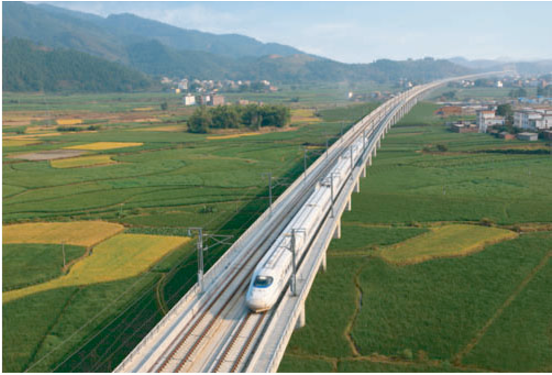
\includegraphics{./images/ch5/rw1.pdf}}
	
	{\it 铁路设计中的问题:列车从直线轨道进入圆弧轨道时,在转换的瞬间,
	
	离心力由零变为一个常数,如果车速较快,会车体和乘客产生很大的冲击。
	
	能否/如何通过更合理的设计,减缓冲击,保证列车运行的安全、舒适?}
\end{center}

\subsubsection{概念}

{\bf 问题:}如何刻画曲线的弯曲程度?

\begin{center}
	\resizebox{!}{5.5cm}{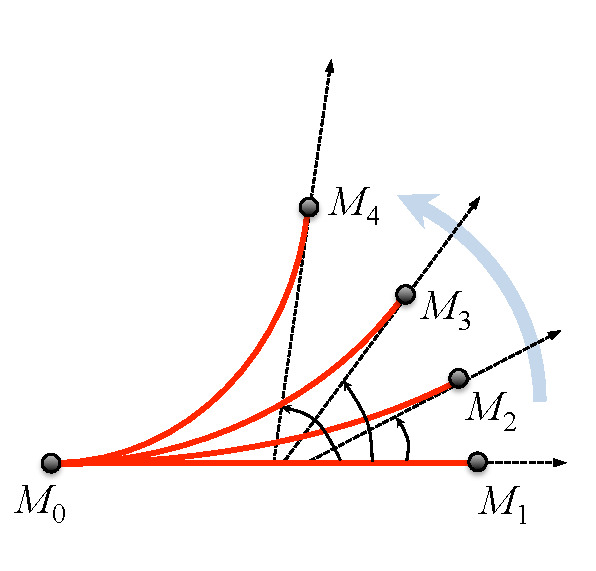
\includegraphics{./images/ch5/curves/c101.pdf}}\quad
	\resizebox{!}{5.5cm}{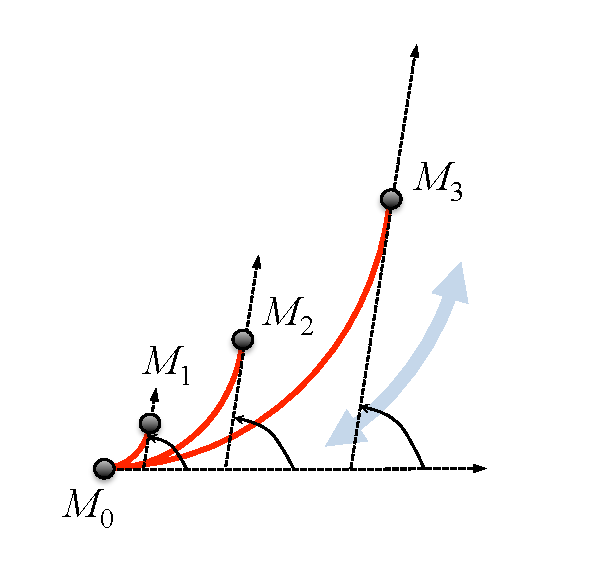
\includegraphics{./images/ch5/curves/c201.pdf}}
\end{center}

\begin{itemize}
  \setlength{\itemindent}{1cm}
  \item 长度相同的曲线,切线转角越大弯曲程度越大
  \item 切线转角相同的曲线,弧长越短弯曲程度越大
\end{itemize}

{\it 曲线的弯曲程度与切线的转角成正比,与弧长成反比}

\begin{thx}
	设曲线$C$光滑且可求长度。 从其上一点$M_0$出发,
	到另一点$M$的弧长为$\Delta s$,切线转角为$\Delta\alpha$。
	 若极限$\lim\limits_{\Delta s\to
	0}\left|\df{\Delta\alpha}{\Delta s}\right|$存在,
	则称之为{\bf 曲线$C$在$M_0$处的曲率:}
	$${K=\lim\limits_{\Delta s\to
	0}\left|\df{\Delta\alpha}{\Delta s}\right|
	=\left|\df{\d\alpha}{\d s}\right|}$$ 
\end{thx}

曲率是曲线上某一点处的切线转角关于弧长的变化率。

% $$K=\df{|y''|}{(1+(y')^2)^{\frac32}}$$

设$y=f(x)$在$x_0$的某邻域内二阶可导,则
\begin{thx}
	$$K=\left|\df{\d\alpha}{\d s}\right|
	 =\df{|y''_{xx}|}{[1+(y'_x)^2]^{3/2}}$$
\end{thx}
 
{\bf 例:}求直线与圆的曲率。

{\bf 例:}求椭圆$x=3\cos t,y=2\sin t\,(0\leq t\leq 2\pi)$
上任意点处的曲率,并指出其中曲率最大的点。

\begin{center}
	\resizebox{!}{4.5cm}{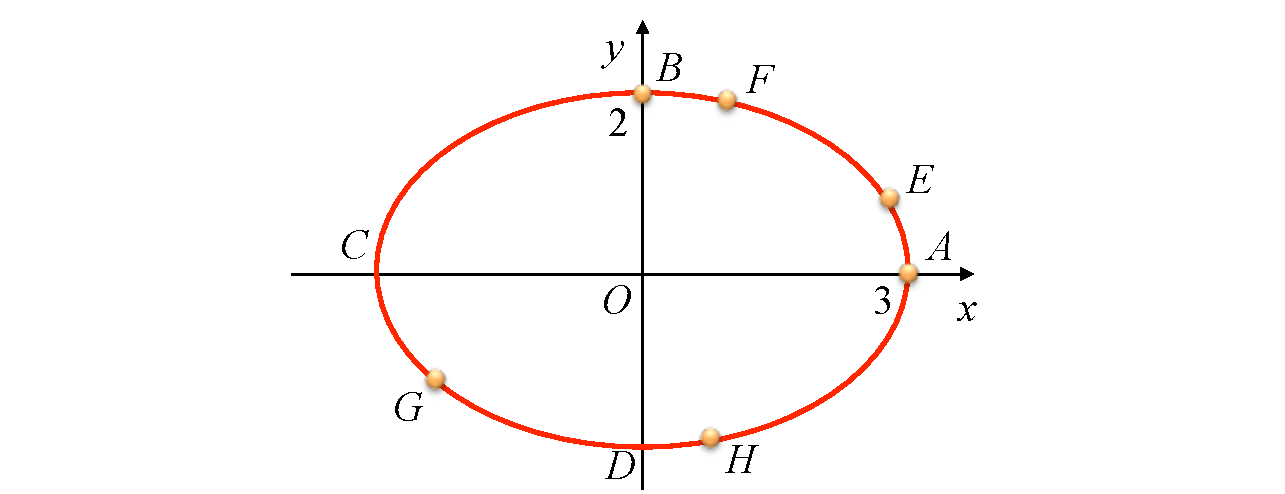
\includegraphics{./images/ch5/ec/newEC/ec01.pdf}}
\end{center}

\begin{thx}
	{\bf 参数方程下的曲率公式:}
	$${K=\df{|x'_ty''_{tt}-x''_{tt}y'_t|}
	{\{[x'_t]^2+[y'_t]^2\}^{3/2}}}$$
	
	{\bf 极坐标下的曲率公式:}
	$$K=\df{|\rho^2+2(\rho')^2-2\rho\rho''|}{[\rho^2+(\rho')^2]^{3/2}}$$
\end{thx}

{\bf 思考:}如何推导出极坐标下的曲率公式?

\subsubsection{曲率圆与曲率的应用}

{\bf 曲率圆:}与给定曲线在凹侧相切,且曲率相同的圆
\ps{曲率圆的圆心称为{\bf 曲率中心}}

\begin{thx}
	{\bf 曲率圆的性质}:曲率圆与给定曲线二阶相切。
\end{thx}

{\bf 思考:}{\b 与已知曲线在给定点处二阶相切的圆一定是其曲率圆吗?(${\bm{\surd}}$)}

{\bf 例:}求曲率圆的方程

\begin{center}
	\resizebox{!}{5cm}{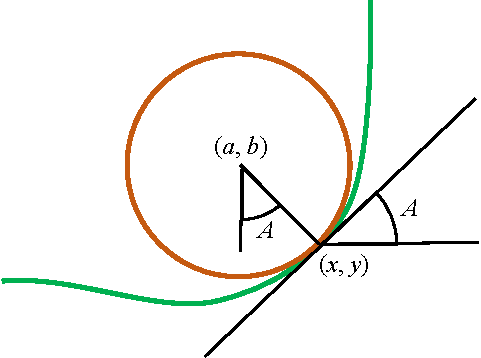
\includegraphics{./images/ch5/curveSphere.pdf}}
\end{center}

[提示]:如图,设曲率圆的圆心为$(a,b)$,$(x,y)$处的导数和二阶导数记为$y',y''$,
显然曲率半径$R=\df1K=\df{[1+(y')^2]^{3/2}}{|y''|}$,为了保持和曲线的凹向一致,
我们将曲率半径定义为有方向的$R=\df{[1+(y')^2]^{3/2}}{y''}$\ps{凹侧的半径为正,
凸侧为负!}。记$(x,y)$处的切线与$x$轴夹角为$A$,则
\begin{align}
	a&=x-R\sin A=x-\df{[1+(y')^2]^{3/2}}{y''}\df{y'}{[1+(y')^2]^{1/2}}
	=x-\df{y'[1+(y')^2]}{y''}\notag\\
	b&=y+R\cos A=y+\df{[1+(y')^2]^{3/2}}{y''}\df1{[1+(y')^2]^{1/2}}
	=y+\df{1+(y')^2}{y''}\notag
\end{align}

\begin{center}
	\resizebox{!}{5.5cm}{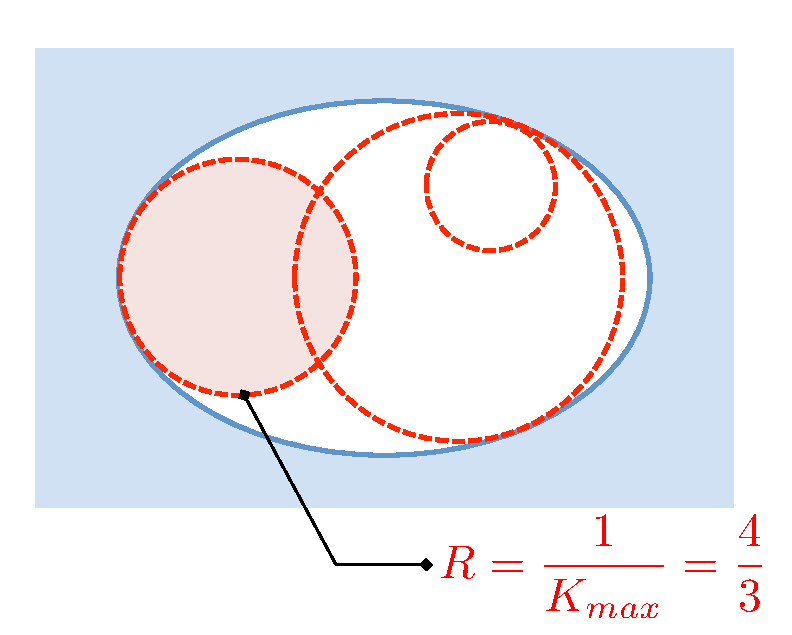
\includegraphics{./images/ch5/SE/S01.pdf}}
\end{center}

{\bf 例:}(加工问题)已知某工件内侧的截痕曲线为椭圆$\df{x^2}9+\df{y^2}4=1$,
若用圆形砂轮对其进行打磨,问该如何选择砂轮的尺寸?

{\bf 注:}利用砂轮磨削一般工件的内表面时,砂轮的半径不应超过工件内表面
的截线上各点处的曲率半径的最小值

{\bf 定律:}质量为$m$的质点以速度$v$通过光滑曲线上一点,所受向心力为
$$F=\df{mv^2}{R},$$
其中$R$为曲线在该点处的曲率半径。

\begin{center}
	\resizebox{!}{3cm}{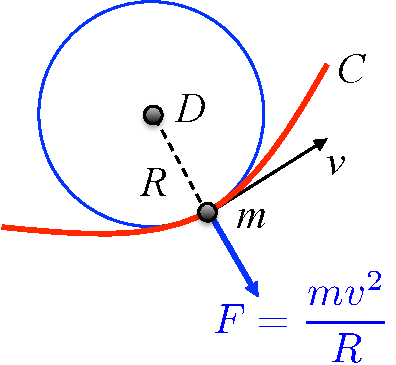
\includegraphics{./images/ch5/flip.pdf}}
\end{center}

{\bf 例:}$\Gamma_1$为射线$y=0,x\leq0$,$\Gamma_2$为椭圆$\df{4(x-2)^2}9+y^2=1$。
使找出一条次数尽可能低的多项式函数曲线$\Gamma_2$,连接$(0,0)$和$(2,1)$,使得最终
完整的曲线曲率连续。

[提示]:$\Gamma_2$在$(2,1)$处的曲率为$-\df49$。
设新的曲线为$\Gamma_3:y=y(x)$,显然
$$y(0)=0,\;y'(0)=0,\;y''(0)=0,$$
$$y(2)=1,\;y'(2)=0,\;y''(2)=-\df49$$
六个条件,意味着至少需要一个$5$次多项式。考虑到$y(0)=y'(0)=y''(0)=0$,
可设$y=ax^3+bx^4+cx^5$,于是
$$
\left\{
\begin{array}{l}
1=8a+16b+32c\\
0=12a+32b+80c\\
-\df49=12a+48b+160c
\end{array}
\right.
$$
行列式非零,方程组解唯一。

\subsubsection{铁路中的缓和曲线}

\begin{center}
	\resizebox{!}{9cm}{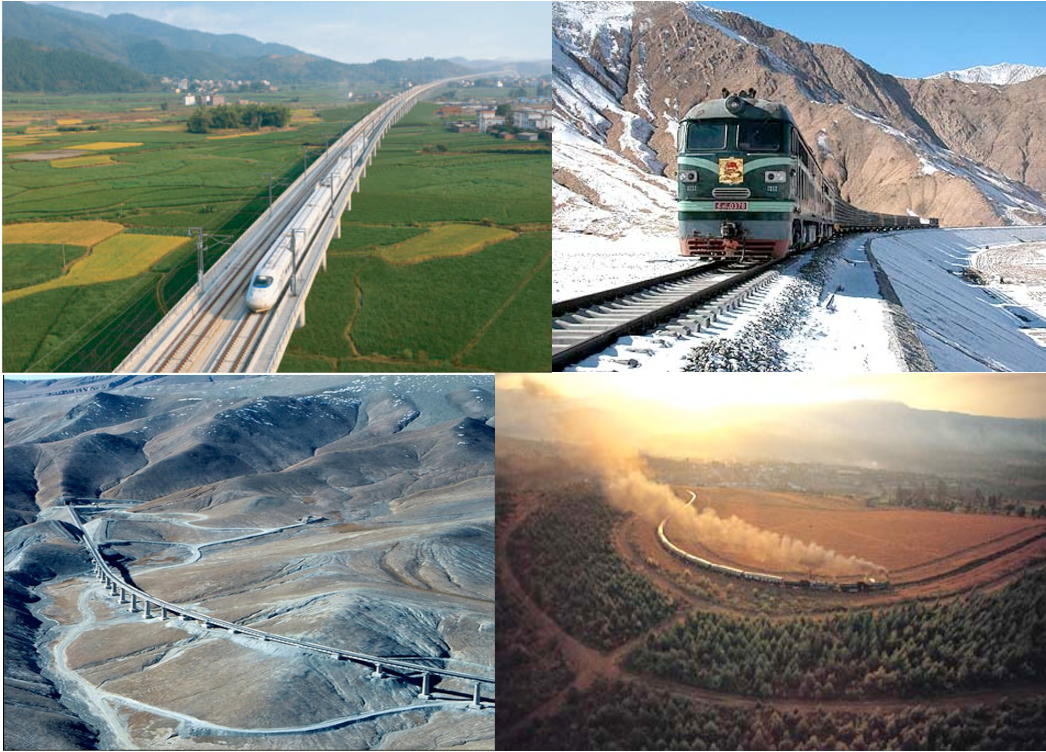
\includegraphics{./images/ch5/railway.pdf}}
\end{center}

{\bf 设计要求:}为了确保列车行驶安全,尽可能保证列车运行时所受向心力的平稳变化

{\bf 常用的缓和曲线:}三次多项式、渐开螺旋线、双纽线、\ldots

{\bf 例:}如图,列车匀速行进,经过一段直线轨道后,将进入半径为$R$的圆弧轨道。为
尽量减少列车行驶中所受的向心力冲击,试确定一个三次多项式函数实现两段轨道的连接。

\begin{center}
	\resizebox{!}{5.2cm}{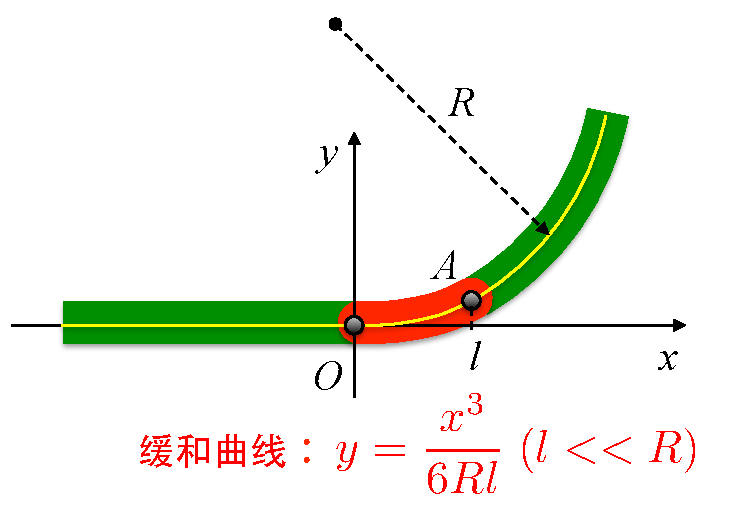
\includegraphics{./images/ch5/rc01.pdf}}
\end{center}

\begin{itemize}
  \item 匀速行驶$v=108km/h$
  \item 列车重量$m=500t$
  \item 圆弧半径$R=1000m$
  \item 缓和曲线长$l=90m$
\end{itemize}

\begin{center}
	\resizebox{!}{4cm}{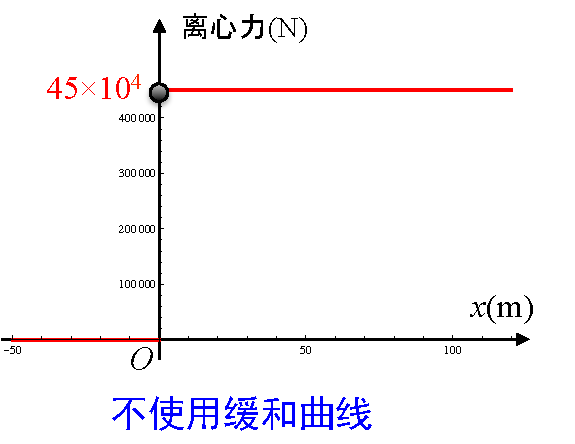
\includegraphics{./images/ch5/f01.pdf}}\quad
	\resizebox{!}{4cm}{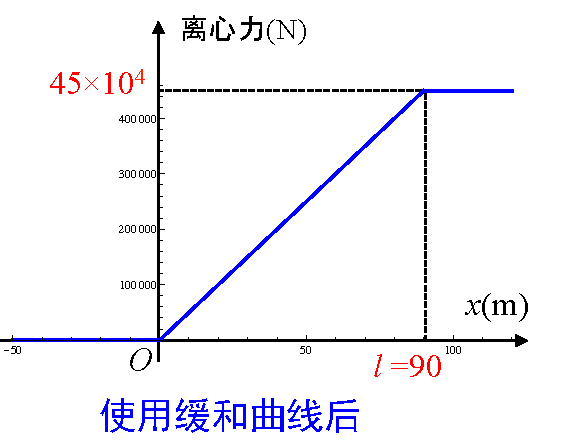
\includegraphics{./images/ch5/f02.pdf}}
\end{center}

类似的问题广泛存在于高速公路、过山车,甚至是飞行器表面的设计中。

\subsection{曲率的应用}

极限是微积分理论体系中最基本也最重要的概念之一,后面我们将要讨论的导数(微分)和
积分的概念都是建立在极限概念之上的,更具体地说,导数和定积分都是特定类型的极限。

在上一章学习了数列极限的基础上,本章我们将进一步讨论更具一般性的函数的极限,二者
的定义和性质,从很多方面来看都是相似的,只是由于函数极限的类型更为丰富,相对而言
有关结论也更为多样,有些性质是数列极限所不具备的。

\begin{ext}
	{\bf 课后作业}
	
	\begin{enumerate}
	  \item 求曲线$y=\ln\cos x$的最小曲率半径。
	  \item 求曲线$x=a\cos^3t,y=b\sin^3t$在$t=t_0$对应点处的曲率。
	  \item 求曲线$x^2+xy+y^2=3$在点$(1,1)$处的曲率半径。
	  \item (选作)推导极坐标形式下曲线$\rho=\rho(\theta)$的曲率公式。
	\end{enumerate}
\end{ext}

\section{小结}

导数为我们提供了研究函数和平面曲线的新的工具。Newton正是因为发明了{\it 流数法
\ps{导数的前身}},才从Kepler三定律推导出了万有引力定律。

本章的内容包含两个大的方面:一是对函数几何形态的研究,涉及:{\it 单调性、最值、极值、
凹凸性、弧长、曲率等}多个方面,由此最终可以对给定的函数给出一个相对
全面的几何刻画,其中很多是在大学之前所不曾接触的;二是{\it 中值定理与Taylor公式},特别是
后者,可以说是微分学中的集大成者,其中蕴含了几乎所有的微分学理论与技巧,从Rolle定理、
Lagrange中值定理、Cauchy中值定理到Taylor中值定理,以及L'Hospital法则,其
内在的统一是学习中需要把握的重点。

在极值、最值、凹凸性等问题中,涉及一些相近而不同的概念,例如:极值点、最值点、拐点、
驻点等,这些概念既相互联系,又有重要的区别,琢磨弄懂它们的异同,能够结合实例有效
地加以区分和应用,是学习的关键。当然,既然是讨论几何问题,对于几何意义和几何特征
的正确把握也是非常重要的。

中值定理的证明问题是本章的难点,从结论出发,构造辅助函数,再验证条件应用中值定理,
是解题的一般思路,但有时如何将结果转换成可以还原的形式,会是相当大的挑战,
为此,有必要掌握一些特定形式(例如:$f'(\xi)+\lambda f(x)$)所对应的辅助函数。
此外,本章两个部分的内容本身并不是相互独立的,事实上,很多结论的推导和证明都需要
同时应用两个部分的结果,特别是从几何上看,中值定理也通常有自身明确的含义,而能够
结合几何意义解决中值问题,可以说才是本章解题的最高境界。

最后,提醒一句,不要迷恋Taylor公式,还是那句话,万能工具虽然万能,但往往不是
效率最高和用起来最简单的一个。